\documentclass[11pt]{article}

\usepackage[a4paper,margin=0.75in]{geometry}
\usepackage{amsmath,amssymb}
\usepackage{graphicx}
\graphicspath{{figures/}{./}}
\usepackage{booktabs}
\usepackage{array}
\usepackage{float}
\usepackage{caption}
\usepackage{hyperref}
\usepackage{enumitem}
\usepackage{xcolor}
\usepackage{listings}
\usepackage{tikz}
\usetikzlibrary{positioning,arrows.meta,shapes.geometric,calc}

\hypersetup{hidelinks}
\setlist{nosep,leftmargin=*}
\renewcommand{\arraystretch}{1.25}
\setlength{\tabcolsep}{4pt}
\setlength{\emergencystretch}{3em}
\setlength{\parindent}{0pt}
\setlength{\parskip}{4pt}
\captionsetup{font=small,labelfont=bf,skip=4pt}
\DeclareCaptionType{diagram}[Diagram][]

\lstset{
language=Python,
basicstyle=\ttfamily\scriptsize,
breaklines=true,
columns=fullflexible,
keepspaces=true,
showstringspaces=false,
frame=single,
rulecolor=\color{black!30},
numbers=left,
numberstyle=\tiny\color{black!50},
numbersep=5pt,
xleftmargin=1.6em,
framexleftmargin=1.6em,
keywordstyle=\color{blue!60!black}\bfseries,
commentstyle=\color{green!40!black}\itshape,
stringstyle=\color{red!50!black}
}

% framed one-line statement used in the manual (centred box)
\newcommand{\qbox}[1]{\begin{center}\fbox{\,#1\,}\end{center}}

\tikzset{
layer/.style={
draw,
rounded corners,
minimum width=1.5cm,
minimum height=0.6cm,
align=center,
fill=blue!10,
font=\scriptsize
},
att/.style={
draw,
rounded corners,
minimum width=1.5cm,
minimum height=0.6cm,
align=center,
fill=green!12,
font=\scriptsize
},
arrow/.style={
-{Latex[length=2mm]},
thin
}
}

\begin{document}

%%%%%%%%%%%%%%%%%%%%%%%%%%%%%%%%%%%%%%%%%%%%%%%%%%%%%%%%%%%%
% TITLE
%%%%%%%%%%%%%%%%%%%%%%%%%%%%%%%%%%%%%%%%%%%%%%%%%%%%%%%%%%%%

\begin{center}

{\large\textbf{Shiv Nadar University Chennai}}

\vspace{2mm}

{\normalsize\textbf{CS3807 -- Deep Learning Laboratory}}

\vspace{2mm}

{\large\textbf{Experiments 8, 9}}

\vspace{1mm}

{\normalsize\textbf{Effect of Attention Type and Attention Position}}

{\normalsize\textbf{in a Pretrained ResNet50}}

\end{center}

\vspace{3mm}

\begin{tabular}{|p{3.4cm}|p{9.0cm}|p{1.4cm}|}
\hline
Degree \& Branch &
B.Tech Artificial Intelligence \& Data Science &
Semester V\\
\hline
Subject Code \& Name &
CS3807 -- Deep Learning Laboratory &
AY: 2026--27\\
\hline
Name & Madhav.S & \\
\hline
Section & AIDS `B' & \\
\hline
Register Number & 24011101066 & \\
\hline
\end{tabular}

%%%%%%%%%%%%%%%%%%%%%%%%%%%%%%%%%%%%%%%%%%%%%%%%%%%%%%%%%%%%
\section*{1. Objective}

The objective of this experiment is to understand how different attention
mechanisms modify a pretrained convolutional network, and how the
\textbf{position at which attention is inserted} influences image
classification performance.

A single pretrained architecture,

\qbox{ResNet50 pretrained on ImageNet}

is used throughout the experiment. The following were investigated:

\begin{itemize}
\item channel attention;
\item spatial attention;
\item sequential channel--spatial attention;
\item lightweight self-attention;
\item different positions for inserting attention within ResNet50;
\item single-stage and multi-stage attention;
\item attention ordering;
\item additional established attention mechanisms; and
\item qualitative interpretation using internal attention maps and Grad-CAM.
\end{itemize}

A single backbone, ResNet50 pretrained on ImageNet, was used throughout on
the TensorFlow Flowers dataset (five classes). Channel, spatial, sequential
channel--spatial, lightweight self-attention, ECA and CBAM modules were
inserted at different stages and compared quantitatively (accuracy,
precision, recall, macro F1, parameters, inference time) and qualitatively
(internal attention maps and Grad-CAM).

The experiment emphasizes that the effectiveness of attention depends not
only on the attention mechanism itself, but also on the characteristics of
the feature representation on which it operates.

\textbf{Scope of this report.} Sixteen models were trained under one fixed
protocol (Section~9.3): the baseline, six attention types at $P_3$, the
position and multi-position variants, the reverse attention order, three
spatial-kernel sizes, and two additional mechanisms (ECA and CBAM). The
report follows the structure suggested in the manual: aim, dataset,
architecture, attention mechanisms, experimental setup, the ablations,
performance and complexity results, training graphs, confusion matrices,
Grad-CAM and internal attention maps, qualitative comparison, the additional
comparison, discussion and conclusion.

%%%%%%%%%%%%%%%%%%%%%%%%%%%%%%%%%%%%%%%%%%%%%%%%%%%%%%%%%%%%
\section*{2. Learning Outcomes}

After completing this experiment, students will be able to:

\begin{enumerate}
\item explain the stage-wise architecture of a pretrained ResNet50;
\item distinguish early, intermediate, and late convolutional features;
\item explain the motivation behind attention mechanisms;
\item implement channel attention;
\item implement spatial attention;
\item implement sequential channel--spatial attention;
\item implement a lightweight self-attention mechanism;
\item insert an attention module at different stages of a pretrained network;
\item analyze the influence of attention position;
\item compare different attention mechanisms under a controlled experimental protocol;
\item analyze classification accuracy and class-wise performance;
\item visualize internal attention maps;
\item generate Grad-CAM explanations;
\item distinguish an internal attention map from a post-hoc explanation map;
\item analyze accuracy--complexity trade-offs; and
\item perform controlled ablation studies.
\end{enumerate}

%%%%%%%%%%%%%%%%%%%%%%%%%%%%%%%%%%%%%%%%%%%%%%%%%%%%%%%%%%%%
\section*{3. Dataset and Experimental Setup}

\subsection*{3.1 Dataset}

\textbf{Dataset: TensorFlow Flowers (\texttt{tf\_flowers})}

The dataset contains 3{,}670 natural RGB flower images in five classes:
daisy, dandelion, roses, sunflowers and tulips. The images contain
variations in:

\begin{itemize}
\item scale;
\item viewpoint;
\item illumination;
\item background clutter;
\item flower size;
\item colour;
\item texture; and
\item object location.
\end{itemize}

These variations make the dataset suitable for studying the behaviour of
attention mechanisms.

\subsection*{3.2 Image Preprocessing and Augmentation}

Every image was resized to

\[
224\times224\times3
\]

and preprocessed with ResNet50's own \texttt{preprocess\_input} function
(RGB to BGR conversion and subtraction of the ImageNet channel means), which
is the procedure expected by the ImageNet-pretrained network.
Random horizontal flip, small rotation, random zoom, random translation and
mild contrast variation were applied to the \emph{training set only}, and
the same augmentation was used for every model. Validation and test images
were only resized and preprocessed.

\begin{center}
\small
\begin{tabular}{|l|l|l|}
\hline
Operation & Keras layer & Setting\\
\hline
Horizontal flip & \texttt{RandomFlip} & horizontal only\\
Small rotation & \texttt{RandomRotation(0.05)} & up to $\pm5\%$ of a full turn ($\pm18^{\circ}$)\\
Random zoom & \texttt{RandomZoom(0.1)} & up to 10\% in or out\\
Random translation & \texttt{RandomTranslation(0.1, 0.1)} & up to 10\% of height and width\\
Mild contrast variation & \texttt{RandomContrast(0.1)} & contrast factor $1\pm0.1$\\
\hline
\end{tabular}
\end{center}

The augmentation pipeline is rebuilt with the same seed for every
experiment, so every model sees the same shuffling and augmentation
sequence and only the model changes.

\subsection*{3.3 Dataset Split}

The same training, validation and testing split was used for every
experiment:

\qbox{$70\% : 15\% : 15\%$ \quad for \quad Training : Validation : Testing}

\textbf{Split.} The images were split by class (stratified) into a fixed
70/15/15 train/validation/test split using seed 42. The exact same samples
were used in every experiment.

The exact same samples were retained in each subset for all ablation
experiments. This is necessary to ensure that differences in performance
are caused by changes in the model rather than changes in the dataset split.

\begin{center}
\small
\begin{tabular}{|l|c|c|c|c|c|c|}
\hline
Split & Images & Daisy & Dandelion & Roses & Sunflowers & Tulips\\
\hline
Training & 2{,}569 & 443 & 629 & 449 & 489 & 559\\
Validation & 550 & 95 & 134 & 96 & 105 & 120\\
Test & 551 & 95 & 135 & 96 & 105 & 120\\
\hline
\end{tabular}
\end{center}

\begin{center}
\includegraphics[width=0.5\linewidth]{fig01_sample_images.pdf}
\captionof{figure}{Sample test images from the five classes (four per class).}
\label{fig:samples}
\end{center}

\textbf{Inference:} The samples show how varied the data is: single close-ups
and whole fields, bright and dark scenes, cluttered backgrounds, and even
people in the frame (sunflower and tulip rows). Some roses (pink bouquets)
and tulips share similar colours and rounded petals, so these two classes
are the likeliest to be confused later on.


%%%%%%%%%%%%%%%%%%%%%%%%%%%%%%%%%%%%%%%%%%%%%%%%%%%%%%%%%%%%
\section*{4. Pretrained Architecture: ResNet50}

ResNet50 pretrained on ImageNet is the only backbone. As the network gets
deeper the spatial resolution falls while the number of channels grows, and
the features move from edges and textures to high-level, class-specific
semantics. The stage dimensions below were verified on the Keras model:

For an input image
\[
I\in\mathbb{R}^{224\times224\times3},
\]
the major ResNet50 stages produce the feature dimensions listed below. The
last column is the number of activations ($H\times W\times C$) a stage hands
to the next one.

\begin{center}
\small
\begin{tabular}{|l|l|c|c|c|r|}
\hline
ResNet50 Stage & Last Keras layer & Blocks & Spatial Resolution & Channels & $H\!\cdot\! W\!\cdot\! C$\\
\hline
Stem + MaxPool & \texttt{pool1\_pool} & -- & $56\times56$ & 64 & 200{,}704\\
conv2\_x & \texttt{conv2\_block3\_out} & 3 & $56\times56$ & 256 & 802{,}816\\
conv3\_x & \texttt{conv3\_block4\_out} & 4 & $28\times28$ & 512 & 401{,}408\\
conv4\_x & \texttt{conv4\_block6\_out} & 6 & $14\times14$ & 1024 & 200{,}704\\
conv5\_x & \texttt{conv5\_block3\_out} & 3 & $7\times7$ & 2048 & 100{,}352\\
\hline
\end{tabular}
\end{center}

As the network becomes deeper

\qbox{Spatial Resolution $\downarrow$}

while

\qbox{Feature Channels $\uparrow$}

and the representation generally progresses from low-level visual
information toward higher-level semantic information. The resolution is
halved at every stage while the number of channels is doubled, so the
number of activations falls from about 0.8 million (conv2\_x) to about 0.1
million (conv5\_x).

\subsection*{4.1 Residual Blocks}

Each stage is built from bottleneck residual blocks: $1\times1$ convolution
(reduce), $3\times3$ convolution, and $1\times1$ convolution (expand), with
batch normalisation and ReLU. A block computes
$y=\mathcal{F}(x,\{W_i\})+x$, where the shortcut $x$ is the identity, or a
$1\times1$ projection in the first block of a stage where the shape changes.
conv2\_x to conv5\_x contain 3, 4, 6 and 3 blocks, i.e.\ 16 blocks and
48 convolutions, which together with the stem convolution and the final
dense layer give the 50 weight layers.

\begin{center}
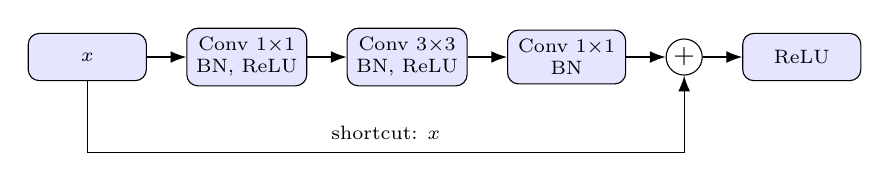
\begin{tikzpicture}[node distance=5mm]
\node[layer](x){$x$};
\node[layer,right=of x](c1){Conv $1{\times}1$\\BN, ReLU};
\node[layer,right=of c1](c2){Conv $3{\times}3$\\BN, ReLU};
\node[layer,right=of c2](c3){Conv $1{\times}1$\\BN};
\node[draw,circle,inner sep=1pt,right=of c3](add){$+$};
\node[layer,right=of add](relu){ReLU};
\draw[arrow](x)--(c1);
\draw[arrow](c1)--(c2);
\draw[arrow](c2)--(c3);
\draw[arrow](c3)--(add);
\draw[arrow](add)--(relu);
\draw[arrow](x.south)--++(0,-0.9)-|(add.south);
\node[above,font=\scriptsize] at ($(x.south)!0.5!(add.south)+(0,-0.9)$){shortcut: $x$};
\end{tikzpicture}
\captionof{diagram}{A bottleneck residual block of ResNet50.}
\end{center}

\textbf{Parameters.} The backbone without its classifier has 23{,}587{,}712
parameters (as reported by Keras). The head used here (GAP, Dropout, Dense
with 5 outputs) adds $2048\times5+5=10{,}245$, so the baseline has
23{,}597{,}957 parameters in total, which is the figure in the result tables.

%%%%%%%%%%%%%%%%%%%%%%%%%%%%%%%%%%%%%%%%%%%%%%%%%%%%%%%%%%%%
\section*{5. ResNet50 Feature Hierarchy and the Role of Attention Position}

\subsection*{5.1 Understanding the Feature Hierarchy}

The approximate interpretation of the different stages is:

\begin{itemize}
\item \textbf{Early features:} edges, colours, orientations, boundaries and
simple textures.
\item \textbf{Intermediate features:} local patterns, repeated structures,
flower parts, petal arrangements and shape information.
\item \textbf{Late features:} high-level object structures and
class-discriminative semantic information.
\end{itemize}

Therefore, the same attention mechanism may produce different behaviour when
inserted at different locations.

\begin{center}
\small
\begin{tabular}{|l|l|p{7.6cm}|}
\hline
Level & Stages & What the features describe\\
\hline
Early & Stem, conv2\_x ($P_1$) & high resolution; edges, colours, textures\\
Intermediate & conv3\_x ($P_2$), conv4\_x ($P_3$) & petal arrangements, flower parts, local shapes\\
Late & conv5\_x ($P_4$) & low resolution; whole-flower, class-specific semantics\\
\hline
\end{tabular}
\end{center}

\subsection*{5.2 Why Attention Position Matters}

Attention is not independent of the features on which it operates. Suppose
an attention module receives
\[
F\in\mathbb{R}^{H\times W\times C}.
\]
The values of $H$, $W$, $C$ and the semantic meaning of the feature tensor
change significantly with network depth. Therefore:

\begin{itemize}
\item \textbf{early-stage attention} operates on high-resolution, low-level
visual information;
\item \textbf{middle-stage attention} operates on intermediate features
containing both spatial and semantic information; and
\item \textbf{late-stage attention} operates on low-resolution, high-level
semantic representations.
\end{itemize}

Thus, both of the following were investigated:

\qbox{Which attention mechanism should be used?}

and

\qbox{Where should the attention mechanism be inserted?}

\subsection*{5.3 Candidate Attention Positions}

Four candidate attention positions are defined in ResNet50:

\[
P_1:\ \text{after conv2\_x},\qquad
P_2:\ \text{after conv3\_x},\qquad
P_3:\ \text{after conv4\_x},\qquad
P_4:\ \text{after conv5\_x}.
\]

\begin{center}
\small
\begin{tabular}{|c|l|c|c|l|}
\hline
Position & Location & Resolution & Channels & Feature type\\
\hline
$P_1$ & After conv2\_x & $56\times56$ & 256 & early\\
$P_2$ & After conv3\_x & $28\times28$ & 512 & intermediate\\
$P_3$ & After conv4\_x & $14\times14$ & 1024 & intermediate\\
$P_4$ & After conv5\_x & $7\times7$ & 2048 & late / semantic\\
\hline
\end{tabular}
\end{center}

For the principal laboratory exercise the focus is on

\qbox{$P_2,\quad P_3,\quad P_4$}

because $P_1$ contains comparatively high-resolution features and may
substantially increase the computational cost of some attention mechanisms.
$P_1$ was nevertheless included in the position study (experiment B1) for
completeness, using the cheap channel--spatial module.

The cost problem is clearest for self-attention, whose attention matrix has
$N\times N$ entries with $N=HW$ (Section~7.4):

\begin{center}
\small
\begin{tabular}{|c|c|c|c|c|}
\hline
Position & Resolution & $N=HW$ & $N^2$ entries & One fp32 matrix per image\\
\hline
$P_1$ & $56\times56$ & 3{,}136 & 9{,}834{,}496 & 39.3~MB\\
$P_2$ & $28\times28$ & 784 & 614{,}656 & 2.5~MB\\
$P_3$ & $14\times14$ & 196 & 38{,}416 & 0.15~MB\\
$P_4$ & $7\times7$ & 49 & 2{,}401 & 0.01~MB\\
\hline
\end{tabular}
\end{center}

This is why self-attention should preferably be introduced at $P_3$ or $P_4$,
and why it was used at $P_3$ here.

%%%%%%%%%%%%%%%%%%%%%%%%%%%%%%%%%%%%%%%%%%%%%%%%%%%%%%%%%%%%
\section*{6. Baseline Model and Insertion of Attention into ResNet50}

\subsection*{6.1 Baseline Model}

The baseline is the pretrained ResNet50 without any additional attention
mechanism.

\begin{center}
\resizebox{0.9\linewidth}{!}{%
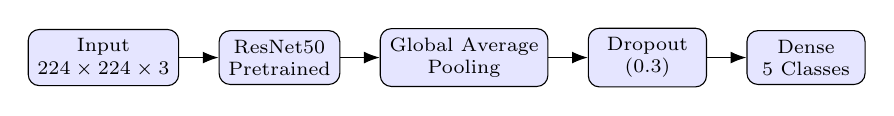
\begin{tikzpicture}[node distance=5mm]
\node[layer](a){Input\\$224\times224\times3$};
\node[layer,right=of a](b){ResNet50\\Pretrained};
\node[layer,right=of b](c){Global Average\\Pooling};
\node[layer,right=of c](d){Dropout\\(0.3)};
\node[layer,right=of d](e){Dense\\5 Classes};
\foreach \x/\y in {a/b,b/c,c/d,d/e}
\draw[arrow](\x)--(\y);
\end{tikzpicture}}
\captionof{diagram}{Baseline model (A0).}
\end{center}

The baseline establishes the reference performance against which the
attention-based models are compared. It is trained with exactly the same
two-stage protocol as every other model and reaches 94.37\% test accuracy.

\subsection*{6.2 Inserting Attention into ResNet50}

For any selected stage $P_k$ the network becomes
\emph{Previous ResNet Stage $\rightarrow$ Attention $\rightarrow$ Next ResNet Stage},
followed by Global Average Pooling, Dropout (0.3) and a Dense layer with 5
softmax neurons. The input and output dimensions of every attention block
were recorded and were identical (for example $14\times14\times1024$
before and after attention at $P_3$), so attention never changed the
feature size.

For example, attention inserted after conv4\_x gives:

\qbox{conv4\_x $\rightarrow$ Attention $\rightarrow$ conv5\_x}

and for channel--spatial attention:

\qbox{conv4\_x $\rightarrow$ Channel Attention $\rightarrow$ Spatial Attention $\rightarrow$ conv5\_x}

In the implementation the pretrained network is cut at the stage-end layers
\texttt{conv2\_block3\_out}, \texttt{conv3\_block4\_out},
\texttt{conv4\_block6\_out} and \texttt{conv5\_block3\_out}. The stage
sub-models share their layers (and pretrained weights) with the backbone,
and the attention layer is placed between two of them. An assertion in the
code checks that the attention block never changes the feature dimensions.
The dimensions immediately before and after every attention block were
recorded:

\begin{center}
\small
\begin{tabular}{|c|l|c|c|}
\hline
Position & After stage & Input $(H,W,C)$ & Output $(H,W,C)$\\
\hline
$P_1$ & conv2\_x & $(56,56,256)$ & $(56,56,256)$\\
$P_2$ & conv3\_x & $(28,28,512)$ & $(28,28,512)$\\
$P_3$ & conv4\_x & $(14,14,1024)$ & $(14,14,1024)$\\
$P_4$ & conv5\_x & $(7,7,2048)$ & $(7,7,2048)$\\
\hline
\end{tabular}
\end{center}

The same input and output shapes were obtained for every module type
(channel, spatial, channel--spatial in both orders, self-attention, combined,
ECA and CBAM) and for the multi-position models, so attention never
modified the spatial or channel dimensions.

\begin{center}
\resizebox{\linewidth}{!}{%
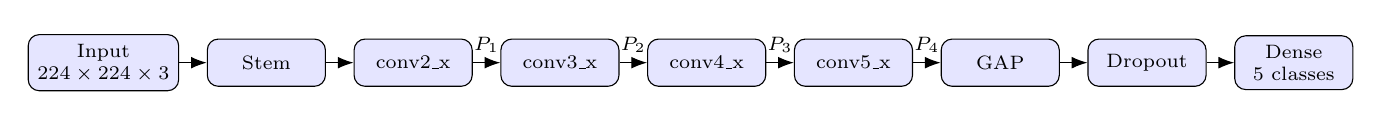
\begin{tikzpicture}[node distance=3.5mm]

\node[layer](a){Input\\$224\times224\times3$};
\node[layer,right=of a](b){Stem};
\node[layer,right=of b](c){conv2\_x};
\node[layer,right=of c](d){conv3\_x};
\node[layer,right=of d](e){conv4\_x};
\node[layer,right=of e](f){conv5\_x};
\node[layer,right=of f](g){GAP};
\node[layer,right=of g](h){Dropout};
\node[layer,right=of h](i){Dense\\5 classes};

\foreach \x/\y in {a/b,b/c,g/h,h/i}
\draw[arrow](\x)--(\y);

\draw[arrow](c)--node[above,font=\scriptsize]{$P_1$}(d);
\draw[arrow](d)--node[above,font=\scriptsize]{$P_2$}(e);
\draw[arrow](e)--node[above,font=\scriptsize]{$P_3$}(f);
\draw[arrow](f)--node[above,font=\scriptsize]{$P_4$}(g);

\end{tikzpicture}}
\end{center}

\captionof{diagram}{ResNet50 with the candidate attention positions $P_1$--$P_4$.}

\textbf{Note:} Attention modules are inserted at the positions marked
$P_1$--$P_4$. $P_3$ is the fixed position for the attention-type study
(Experiment 1).


%%%%%%%%%%%%%%%%%%%%%%%%%%%%%%%%%%%%%%%%%%%%%%%%%%%%%%%%%%%%
\section*{7. Attention Mechanisms}

Every module takes a feature tensor $F\in\mathbb{R}^{H\times W\times C}$ and
returns a tensor of the same shape. The parameter counts below are for
$P_3$ ($C=1024$) and agree exactly with the counts measured on the trained
models.

\subsection*{7.1 Channel Attention}

Channel attention determines the relative importance of the different
feature channels. Global average pooling first generates a channel
descriptor $z\in\mathbb{R}^{C}$, which is transformed by two learnable
layers, with reduction ratio $r=16$:

\[
z_c=\frac{1}{HW}\sum_{i=1}^{H}\sum_{j=1}^{W}F(i,j,c),\qquad
M_c(F)=\sigma\left(W_2\,\delta(W_1 z)\right),\qquad
F_c=F\odot M_c(F).
\]

Here $\delta(\cdot)$ is the ReLU, $\sigma(\cdot)$ the sigmoid, $W_1$ reduces
the channel representation ($C\rightarrow C/r$) and $W_2$ restores it
($C/r\rightarrow C$). Channel attention attempts to answer:

\qbox{Which feature channels are important?}

The reduction ratio $r=16$ was used as the default throughout and was not
treated as a separate ablation. At $P_3$ the module has
$(1024\cdot64+64)+(64\cdot1024+1024)=132{,}160$ parameters. This module is the
Squeeze-and-Excitation (SE) formulation (see Section~7.6).

\subsection*{7.2 Spatial Attention}

Spatial attention determines which spatial regions should receive greater
importance. Average and maximum pooling across the channels give two
$H\times W\times1$ maps, which are concatenated and passed through a
$7\times7$ convolution:

\[
F_{\mathrm{avg}}=\mathrm{Mean}_c(F),\quad
F_{\mathrm{max}}=\mathrm{Max}_c(F),\quad
F_s=[F_{\mathrm{avg}}\,\|\,F_{\mathrm{max}}],
\]
\[
M_s(F)=\sigma\left(\mathrm{Conv}_{7\times7}(F_s)\right)\in\mathbb{R}^{H\times W\times1},\qquad
F_s'=F\odot M_s(F).
\]

Spatial attention answers:

\qbox{Which spatial locations are important?}

The $7\times7$ convolution maps two input channels to one, so it has only
$7\cdot7\cdot2+1=99$ parameters regardless of the number of channels
(19 and 51 for the $3\times3$ and $5\times5$ kernels of Experiment~5).

\subsection*{7.3 Sequential Channel--Spatial Attention}

Channel and spatial attention can be applied sequentially. First
$F_c=M_c(F)\odot F$, then $F_{cs}=M_s(F_c)\odot F_c$:

\qbox{$F\rightarrow$ Channel Attention $\rightarrow$ Spatial Attention $\rightarrow F_{cs}$}

This arrangement first determines ``what is important'' and then
``where it is important''. The reverse order (spatial first,
$F\rightarrow M_s\rightarrow M_c$) was used for Experiment~4. A simplified
diagram is shown below.

\begin{center}
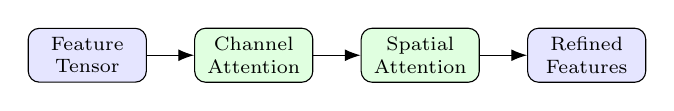
\begin{tikzpicture}[node distance=6mm]
\node[layer](f){Feature\\Tensor};
\node[att,right=of f](c){Channel\\Attention};
\node[att,right=of c](s){Spatial\\Attention};
\node[layer,right=of s](o){Refined\\Features};
\foreach \x/\y in {f/c,c/s,s/o}
\draw[arrow](\x)--(\y);
\end{tikzpicture}
\captionof{diagram}{Sequential channel--spatial attention (Channel $\rightarrow$ Spatial).}
\end{center}

With both modules at $P_3$ the added parameters are $132{,}160+99=132{,}259$,
and the reverse order has exactly the same count.

\subsection*{7.4 Lightweight Self-Attention}

Self-attention allows spatial locations to interact directly with other
spatial locations. The feature map is flattened to $X\in\mathbb{R}^{N\times C}$
with $N=HW$; the query, key and value matrices are $Q=XW_Q$, $K=XW_K$,
$V=XW_V$, and

\[
A=\mathrm{softmax}\!\left(\frac{QK^{T}}{\sqrt{d}}\right),\qquad
Y=AV,\qquad
F_{SA}=F+\gamma\,\mathrm{reshape}(Y),
\]

where $\gamma$ is a learnable scale initialised to 0 and $d=C/8$ is the
query/key size. It attempts to answer:

\qbox{Which spatial features are related to other spatial features?}

At $P_3$ the attention matrix $A$ is $196\times196$, $d=128$, and the module
has $W_Q,W_K\in\mathbb{R}^{1024\times128}$, $W_V\in\mathbb{R}^{1024\times1024}$
(no biases) and the scalar $\gamma$, i.e.\ $2\cdot131{,}072+1{,}048{,}576+1=1{,}310{,}721$
parameters. Because $A$ has $N\times N$ entries, its computational and memory
requirements increase rapidly as $N=HW$ increases (Section~5.3), so
self-attention was introduced at $P_3$.

\subsection*{7.5 Combined Attention (A5)}

\textbf{Combined attention} (A5) applies channel, spatial and self-attention
one after another, $F\rightarrow M_c\rightarrow M_s\rightarrow F_{SA}$. Its
parameter count is the sum of the three modules,
$132{,}160+99+1{,}310{,}721=1{,}442{,}980$.

\subsection*{7.6 Additional Mechanisms: ECA and CBAM}

The manual asks for at least two additional mechanisms from SE, ECA, CBAM,
Coordinate Attention and lightweight self-attention. SE (the channel module)
and self-attention are already part of the main study; \textbf{ECA} and
\textbf{CBAM} were added as the two further established mechanisms.

\textbf{Additional mechanisms.} \emph{ECA} replaces the two dense layers of
channel attention by a single 1-D convolution across neighbouring channels
(kernel size 5 for 1024 channels, no dimensionality reduction).
\emph{CBAM} computes channel attention from both average- and max-pooled
descriptors through a shared MLP, followed by $7\times7$ spatial attention.
The channel-attention module above is the Squeeze-and-Excitation (SE)
formulation, so ``Channel'' and ``SE'' refer to the same model in all
tables and plots.

\medskip
Formally, ECA replaces $W_2\delta(W_1z)$ by a one-dimensional convolution
of the descriptor $z$ over neighbouring channels,
$M_c^{\mathrm{ECA}}(F)=\sigma(\mathrm{Conv1D}_k(z))$, with the adaptive
kernel size $k=\left|\frac{\log_2C+b}{\gamma}\right|_{\mathrm{odd}}$
($\gamma=2$, $b=1$), which gives $k=5$ for $C=1024$ and therefore 5
parameters. CBAM uses a shared MLP on both pooled descriptors,
$M_c(F)=\sigma\big(W_2\delta(W_1z_{\mathrm{avg}})+W_2\delta(W_1z_{\mathrm{max}})\big)$,
and then the same $7\times7$ spatial module, so it has
$132{,}160+99=132{,}259$ parameters at $P_3$.

\subsection*{7.7 Summary of the Modules}

\begin{center}
\small
\begin{tabular}{|l|l|l|r|}
\hline
Module & Question it answers & Operates on & Parameters at $P_3$\\
\hline
Channel / SE & which channels matter & pooled channel vector & 132{,}160\\
Spatial ($7\times7$) & which locations matter & channel-pooled $H\times W$ maps & 99\\
Channel $\rightarrow$ Spatial & what, then where & both & 132{,}259\\
Spatial $\rightarrow$ Channel & where, then what & both & 132{,}259\\
Self-attention & which positions relate & all $N\times N$ position pairs & 1{,}310{,}721\\
Combined (A5) & all three & all of the above & 1{,}442{,}980\\
ECA & which channels matter (local) & 1-D conv over channels & 5\\
CBAM & what, then where (avg + max) & both & 132{,}259\\
\hline
\end{tabular}
\end{center}


%%%%%%%%%%%%%%%%%%%%%%%%%%%%%%%%%%%%%%%%%%%%%%%%%%%%%%%%%%%%
\section*{8. Transfer-Learning Strategy, Loss Function and Evaluation Metrics}

\subsection*{8.1 Transfer-Learning Strategy}

ImageNet pretrained weights were used. The recommended ten-step strategy was
followed exactly:

\begin{center}
\small
\begin{tabular}{|c|l|p{8.6cm}|}
\hline
Step & Requirement & Implementation\\
\hline
1 & Load ResNet50 with ImageNet weights & \texttt{keras.applications.ResNet50(weights="imagenet")}\\
2 & Remove the ImageNet classification layer & \texttt{include\_top=False}\\
3 & Insert the selected attention module & between the stage sub-models at $P_k$\\
4 & Add Global Average Pooling & \texttt{GlobalAveragePooling2D} (2048-d vector at $7\times7\times2048$)\\
5 & Add Dropout & rate 0.3\\
6 & Add a Dense layer with five outputs & Dense(5, softmax)\\
7 & Initially freeze the pretrained layers & stage 1: all ResNet50 layers frozen\\
8 & Train the new layers & attention + classifier, Adam, LR $=10^{-3}$, 10 epochs\\
9 & Unfreeze the final ResNet50 stage & conv5\_x unfrozen, BatchNorm layers kept frozen\\
10 & Fine-tune with a smaller learning rate & Adam, LR $=10^{-4}$, 10 epochs (within $10^{-5}$ to $10^{-4}$)\\
\hline
\end{tabular}
\end{center}

The initial learning rate for the new layers is $10^{-3}$ and fine-tuning uses
the smaller $10^{-4}$. The exact values were kept identical for all
controlled comparisons. The complete setting is summarised below.

\begin{center}
\begin{tabular}{|l|p{11.5cm}|}
\hline
Item & Setting (identical for every model)\\
\hline
Backbone & ResNet50, ImageNet weights, original classifier removed\\
Classifier & Global Average Pooling $\rightarrow$ Dropout (0.3) $\rightarrow$ Dense (5, softmax)\\
Stage 1 & backbone frozen; attention and classifier trained, Adam, LR $=10^{-3}$, 10 epochs\\
Stage 2 & conv5\_x unfrozen (BatchNorm layers kept frozen), Adam, LR $=10^{-4}$, 10 epochs\\
Other & batch size 32, categorical cross-entropy, random seed 42, NVIDIA Tesla T4 GPU\\
\hline
\end{tabular}
\end{center}

\subsection*{8.2 Loss Function}

For the five-class problem, categorical cross-entropy was used. For $N$
samples,

\[
\mathcal{L}_{CE}=-\frac{1}{N}\sum_{i=1}^{N}\sum_{c=1}^{5}y_{i,c}\log\hat{y}_{i,c},
\]

where $y_{i,c}$ is the ground-truth (one-hot) label and $\hat{y}_{i,c}$ is the
predicted probability. The same loss formulation was used for every attention
comparison.

\subsection*{8.3 Evaluation Metrics}

The following quantitative metrics were reported for every model:
classification accuracy; macro precision; macro recall; macro F1-score;
number of trainable parameters; total number of parameters; and average
inference time per image. For class $c$,

\[
\mathrm{Precision}_c=\frac{TP_c}{TP_c+FP_c},\qquad
\mathrm{Recall}_c=\frac{TP_c}{TP_c+FN_c},\qquad
F1_c=2\,\frac{\mathrm{Precision}_c\,\mathrm{Recall}_c}{\mathrm{Precision}_c+\mathrm{Recall}_c},
\]

and the macro F1 is the unweighted mean of $F1_c$ over the classes.

Accuracy, macro precision, macro recall and macro F1 were computed on the
test set, with $\mathrm{Macro\ F1}=\frac{1}{C}\sum_{c=1}^{C}F1_c$ and
$C=5$. Trainable parameters are counted in the fine-tuning state (attention
+ conv5\_x + classifier), total parameters include the whole network, and
inference time is the average time per image over the test set (batches of 32).
Since the test set has 551 images, \textbf{one image equals about 0.18
percentage points}; differences of a few images are within what a re-run
could change.

Inference time was measured as the median of three passes over the test set
after one warm-up batch.

%%%%%%%%%%%%%%%%%%%%%%%%%%%%%%%%%%%%%%%%%%%%%%%%%%%%%%%%%%%%
\section*{9. Experimental Protocol and Experiment Plan}

\subsection*{9.1 Experimental Protocol}

To ensure a fair comparison, all ablation experiments used identical
settings, and only the experimental factor under investigation was changed:

\begin{center}
\small
\begin{tabular}{|l|p{10.6cm}|}
\hline
Kept identical & How it was ensured\\
\hline
Training, validation and testing images & one stratified 70/15/15 split (seed 42), computed once and reused by every experiment\\
Random seed & seed 42 is set before every model is built; the training pipeline is rebuilt with the same seed\\
Image preprocessing & ResNet50 \texttt{preprocess\_input} on $224\times224$ images\\
Augmentation & the same five augmentation layers, training set only\\
Backbone and classifier & ImageNet ResNet50, GAP $\rightarrow$ Dropout (0.3) $\rightarrow$ Dense (5)\\
Optimizer and batch size & Adam, batch size 32\\
Epochs and learning-rate schedule & 10 + 10 epochs, LR $10^{-3}$ then $10^{-4}$ (no decay)\\
Fine-tuning procedure & conv5\_x unfrozen, BatchNorm frozen\\
Evaluation metrics & the same test tensor and the same metric functions\\
\hline
\end{tabular}
\end{center}

For example, when studying attention position

\qbox{Only Attention Position Should Change}

and when studying attention type

\qbox{Only Attention Type Should Change.}

GPU kernels are not completely deterministic, so the same seed does not
guarantee bit-identical numbers on a re-run; this is one more reason to read
small differences with care (Section~8.3).

\subsection*{9.2 Minimum Mandatory Ablation Set}

If laboratory time is limited, a minimum set of ten items must be completed.
All of them were completed:

\begin{center}
\small
\begin{tabular}{|c|l|p{6.6cm}|}
\hline
\# & Required item & Where it is reported\\
\hline
1 & Baseline ResNet50 & A0, Section~10\\
2 & Channel attention at $P_3$ & A1, Section~10\\
3 & Spatial attention at $P_3$ & A2, Section~10\\
4 & Channel+Spatial attention at $P_3$ & A3 / B3, Sections~10--11\\
5 & Channel+Spatial attention at $P_2$ & B2, Section~11\\
6 & Channel+Spatial attention at $P_4$ & B4, Section~11\\
7 & Self-attention at $P_3$ & A4, Section~10\\
8 & Grad-CAM: baseline vs.\ one selected model & Figure~\ref{fig:gc}, Section~20.5\\
9 & Spatial-attention visualization at $P_2$, $P_3$, $P_4$ & Figure~\ref{fig:pos}, Section~20.6\\
10 & Graphical comparison of the attention models & Figures~\ref{fig:accbar}--\ref{fig:f1time}, Section~18\\
\hline
\end{tabular}
\end{center}

This minimum set allows the study of

\qbox{Attention Type}

and

\qbox{Attention Position}

\subsection*{9.3 List of All Trained Models}

\begin{center}
\small
\begin{tabular}{|l|l|l|c|l|}
\hline
Run ID & Model & Attention & Position & Used for\\
\hline
\texttt{baseline} & A0 & none & -- & Exp.~1, comparison\\
\texttt{C\_P3} & A1 & Channel / SE & $P_3$ & Exp.~1, comparison\\
\texttt{S\_P3} & A2 & Spatial ($7\times7$) & $P_3$ & Exp.~1, 5, comparison\\
\texttt{CS\_P3} & A3, B3 & Channel $\rightarrow$ Spatial & $P_3$ & Exp.~1--4 (selected model)\\
\texttt{SA\_P3} & A4 & Self-attention & $P_3$ & Exp.~1, comparison\\
\texttt{CSA\_P3} & A5 & Channel, Spatial, Self & $P_3$ & Exp.~1\\
\texttt{CS\_P1} & B1 & Channel $\rightarrow$ Spatial & $P_1$ & Exp.~2\\
\texttt{CS\_P2} & B2 & Channel $\rightarrow$ Spatial & $P_2$ & Exp.~2\\
\texttt{CS\_P4} & B4 & Channel $\rightarrow$ Spatial & $P_4$ & Exp.~2, 3\\
\texttt{CS\_P3P4} & -- & Channel $\rightarrow$ Spatial & $P_3+P_4$ & Exp.~3\\
\texttt{CS\_P2P3P4} & -- & Channel $\rightarrow$ Spatial & $P_2+P_3+P_4$ & Exp.~3 (extended)\\
\texttt{SC\_P3} & -- & Spatial $\rightarrow$ Channel & $P_3$ & Exp.~4\\
\texttt{S\_P3\_k3} & -- & Spatial ($3\times3$) & $P_3$ & Exp.~5\\
\texttt{S\_P3\_k5} & -- & Spatial ($5\times5$) & $P_3$ & Exp.~5\\
\texttt{ECA\_P3} & -- & ECA & $P_3$ & additional task\\
\texttt{CBAM\_P3} & -- & CBAM & $P_3$ & additional task\\
\hline
\end{tabular}
\end{center}

The Channel+Spatial model at $P_3$ (\texttt{CS\_P3}) is the ``selected
attention-based ResNet50'' used for the confusion matrix and the Grad-CAM
comparison.

\subsection*{9.4 Additional Student Exploration}

Two mechanisms beyond the basic set, ECA and CBAM, were integrated with the
same ResNet50 backbone, keeping the same dataset split, preprocessing,
augmentation, optimizer, epochs, fine-tuning strategy and attention position
($P_3$). The investigation includes both a quantitative comparison
(Section~15) and a qualitative comparison (Figure~\ref{fig:qual2}).


%%%%%%%%%%%%%%%%%%%%%%%%%%%%%%%%%%%%%%%%%%%%%%%%%%%%%%%%%%%%
\section*{10. Experiment 1: Attention-Type Ablation (Position $P_3$)}

The first experiment studies the effect of different types of attention. The
attention position is fixed at

\qbox{$P_3$ = after conv4\_x}

for all models, and the following were compared:

\begin{center}
\small
\begin{tabular}{|l|c|c|c|}
\hline
Model & Channel & Spatial & Self-Attention\\
\hline
A0: Baseline ResNet50 & -- & -- & --\\
A1: Channel Attention & $\checkmark$ & -- & --\\
A2: Spatial Attention & -- & $\checkmark$ & --\\
A3: Channel+Spatial & $\checkmark$ & $\checkmark$ & --\\
A4: Self-Attention & -- & -- & $\checkmark$\\
A5: Combined Attention & $\checkmark$ & $\checkmark$ & $\checkmark$\\
\hline
\end{tabular}
\end{center}

This experiment investigates:

\qbox{How does attention type affect model performance?}

The following were kept identical: dataset split; preprocessing;
augmentation; optimizer; learning-rate schedule; epochs; batch size;
backbone; classifier; attention position; and evaluation procedure.

\begin{center}
\small
\begin{tabular}{|l|c|c|c|c|c|c|}
\hline
Model & Acc. (\%) & Precision & Recall & Macro F1 & Parameters & Time (ms)\\
\hline
A0: Baseline ResNet50 & \textbf{94.37} & 0.9465 & 0.9421 & 0.9436 & 23{,}597{,}957 & 7.67\\
A1: Channel Attention & 93.47 & 0.9373 & 0.9316 & 0.9339 & 23{,}730{,}117 & 7.66\\
A2: Spatial Attention & 93.65 & 0.9411 & 0.9338 & 0.9368 & 23{,}598{,}056 & 8.42\\
A3: Channel+Spatial & 93.83 & 0.9413 & 0.9357 & 0.9370 & 23{,}730{,}216 & 7.70\\
A4: Self-Attention & 94.19 & 0.9453 & 0.9387 & 0.9410 & 24{,}908{,}678 & 8.20\\
A5: Combined Attention & 91.65 & 0.9181 & 0.9139 & 0.9154 & 25{,}040{,}937 & 7.74\\
\hline
\end{tabular}
\end{center}

\textbf{Inference:} None of the attention variants beat the plain ResNet50.
Self-attention comes closest (one image fewer than the baseline), and the
single modules (A1--A3) are about 0.5--0.9 points below it. The clear
outlier is the combined model A5, which combines the three modules, adds 1.44M
parameters and loses 2.7 points (505 versus 520 correct images). With only
2{,}569 training images, a bigger attention block seems to give the network
more to overfit rather than more to use.

%%%%%%%%%%%%%%%%%%%%%%%%%%%%%%%%%%%%%%%%%%%%%%%%%%%%%%%%%%%%
\section*{11. Experiment 2: Attention-Position Ablation (Channel $\rightarrow$ Spatial)}

The second experiment investigates the influence of the position of
attention. The attention type is fixed as

\qbox{Channel Attention $\rightarrow$ Spatial Attention}

and exactly the same module is inserted at different stages (B1--B4). The
study asks whether attention is more beneficial for high-resolution
low-level features, intermediate representations, or low-resolution semantic
features. The principal question is:

\qbox{How does the location of attention influence performance?}

\begin{center}
\small
\begin{tabular}{|l|c|c|c|c|c|c|c|}
\hline
Experiment & Resolution & Acc. (\%) & Precision & Recall & Macro F1 & Parameters & Time (ms)\\
\hline
B1: after conv2\_x ($P_1$) & $56\times56\times256$ & 92.56 & 0.9245 & 0.9271 & 0.9252 & 23{,}606{,}520 & 8.40\\
B2: after conv3\_x ($P_2$) & $28\times28\times512$ & 92.20 & 0.9263 & 0.9196 & 0.9206 & 23{,}631{,}368 & 8.37\\
B3: after conv4\_x ($P_3$) & $14\times14\times1024$ & \textbf{93.83} & 0.9413 & 0.9357 & 0.9370 & 23{,}730{,}216 & 7.70\\
B4: after conv5\_x ($P_4$) & $7\times7\times2048$ & 93.65 & 0.9405 & 0.9369 & 0.9367 & 24{,}124{,}520 & 8.41\\
\hline
\end{tabular}
\end{center}

\medskip
The cost of the identical module grows with the stage because its dense
layers scale with the number of channels, about $2C^2/r$ weights:

\begin{center}
\small
\begin{tabular}{|c|c|c|c|c|}
\hline
Position & Channels $C$ & Channel module & Spatial module & Total added\\
\hline
$P_1$ & 256 & 8{,}464 & 99 & 8{,}563\\
$P_2$ & 512 & 33{,}312 & 99 & 33{,}411\\
$P_3$ & 1024 & 132{,}160 & 99 & 132{,}259\\
$P_4$ & 2048 & 526{,}464 & 99 & 526{,}563\\
\hline
\end{tabular}
\end{center}

Each step doubles $C$ and multiplies the added parameters by about four. The
counts equal the differences between the parameter totals of the trained
models and the baseline (23{,}597{,}957).

\textbf{Inference:} The middle-to-late positions work best: $P_3$ is on top
(93.83\%) with $P_4$ right behind (93.65\%), while the early positions $P_1$
and $P_2$ are 1.3--1.6 points lower. Early features are edges and textures
that are all useful, so there is little for attention to select, whereas
deeper features are more class-specific. $P_4$ also costs four times as
many extra parameters as $P_3$ (526{,}563 versus 132{,}259) because it
works on 2048 channels, for no gain, so $P_3$ is the best trade-off here.

%%%%%%%%%%%%%%%%%%%%%%%%%%%%%%%%%%%%%%%%%%%%%%%%%%%%%%%%%%%%
\section*{12. Experiment 3: Multiple Attention Positions (Channel $\rightarrow$ Spatial)}

Attention may also be inserted at more than one ResNet50 stage. The
following were compared: attention only at $P_3$, attention only at $P_4$,
and attention at $P_3+P_4$. As an extended experiment, $P_2+P_3+P_4$ was
also evaluated. The purpose is to investigate whether applying attention
repeatedly provides sufficient performance improvement to justify the
additional parameters, computation, memory, training time and inference
time. The question to be answered experimentally is:

\qbox{Is attention at more locations necessarily more effective?}

Parameters were counted from the models, memory is the peak GPU memory
reported by the TensorFlow allocator during training, and computation is
reflected by the measured training and inference time.

\begin{center}
\small
\begin{tabular}{|l|c|c|c|c|c|c|}
\hline
Model & Acc. (\%) & Macro F1 & Added params & Train (s) & Peak GPU (MB) & Inf. (ms)\\
\hline
Only $P_3$ & \textbf{93.83} & 0.9370 & 132{,}259 & 858 & 1{,}322 & 7.70\\
Only $P_4$ & 93.65 & 0.9367 & 526{,}563 & 848 & 2{,}577 & 8.41\\
$P_3+P_4$ & 93.47 & 0.9346 & 658{,}822 & 862 & 2{,}801 & 8.56\\
$P_2+P_3+P_4$ (extended) & 93.47 & 0.9346 & 692{,}233 & 867 & 3{,}409 & 8.69\\
\hline
\end{tabular}
\end{center}

\medskip
The added parameters of a multi-position model are simply the sum of its
modules: $132{,}259+526{,}563=658{,}822$ for $P_3+P_4$, and
$33{,}411+132{,}259+526{,}563=692{,}233$ for $P_2+P_3+P_4$.

\textbf{Inference:} Adding attention at more stages did not help. Accuracy
drifts down from 93.83\% to 93.47\% (two images) while the extra
parameters grow five-fold, GPU memory rises from about 1.3~GB to
3.4~GB and inference time goes up by about 1~ms. Training time barely
changes (around 14 minutes for every model). So attention at more locations is not necessarily more
effective, and the single $P_3$ module gives the best return.

%%%%%%%%%%%%%%%%%%%%%%%%%%%%%%%%%%%%%%%%%%%%%%%%%%%%%%%%%%%%
\section*{13. Experiment 4: Attention Order (at $P_3$)}

The sequence in which channel and spatial attention are applied may
influence the resulting features. Channel $\rightarrow$ Spatial,
$F\rightarrow M_c\rightarrow M_s$, was compared against Spatial
$\rightarrow$ Channel, $F\rightarrow M_s\rightarrow M_c$, at the same
insertion position $P_3$. The aim is to determine whether selecting
informative feature channels before selecting spatial regions produces
behaviour different from selecting spatial regions first.

\begin{center}
\small
\begin{tabular}{|l|c|c|c|c|c|}
\hline
Order & Acc. (\%) & Precision & Recall & Macro F1 & Time (ms)\\
\hline
Channel $\rightarrow$ Spatial ($F\rightarrow M_c\rightarrow M_s$) & 93.83 & 0.9413 & 0.9357 & 0.9370 & 7.70\\
Spatial $\rightarrow$ Channel ($F\rightarrow M_s\rightarrow M_c$) & 93.83 & 0.9407 & 0.9395 & 0.9396 & 8.27\\
\hline
\end{tabular}
\end{center}

\textbf{Inference:} The order made no real difference: accuracy is
identical, and spatial-first has a slightly better recall and macro F1
(+0.26 points, about one or two images). Both models have exactly the same
parameters (23{,}730{,}216) and perform the same operations, yet their
timings differ by 0.6~ms, which shows that timing gaps below about 1~ms in
this report are measurement noise rather than real cost.

%%%%%%%%%%%%%%%%%%%%%%%%%%%%%%%%%%%%%%%%%%%%%%%%%%%%%%%%%%%%
\section*{14. Experiment 5: Spatial-Attention Kernel Size (at $P_3$)}

The receptive field used to generate the spatial attention map may
influence the result. Spatial attention at $P_3$ was evaluated for
$k\in\{3,5,7\}$ with the same position and training protocol. On the
$14\times14$ map a window covers a different share of the image:

\begin{center}
\small
\begin{tabular}{|c|c|c|c|}
\hline
Kernel & Window area & Share of the $14\times14$ map & Parameters\\
\hline
$3\times3$ & 9 cells & 4.6\% & 19\\
$5\times5$ & 25 cells & 12.8\% & 51\\
$7\times7$ & 49 cells & 25.0\% & 99\\
\hline
\end{tabular}
\end{center}

\begin{center}
\begin{tabular}{|c|c|c|c|}
\hline
Spatial Kernel & Accuracy (\%) & Macro F1 & Inference Time (ms)\\
\hline
$3\times3$ & 92.01 & 0.9157 & 8.30\\
$5\times5$ & 93.10 & 0.9321 & 8.35\\
$7\times7$ & \textbf{93.65} & \textbf{0.9368} & 8.42\\
\hline
\end{tabular}
\end{center}

\textbf{Inference:} Accuracy and macro F1 both rise steadily with the
kernel size, from 92.01\% to 93.65\% (nine more images correct). A
$3\times3$ window only sees a tiny part of the $14\times14$ map, while a
$7\times7$ window collects much greater context before deciding which
locations matter. The price is negligible (about 80 more parameters and
0.1~ms), so a larger kernel is a useful increase in context here.

%%%%%%%%%%%%%%%%%%%%%%%%%%%%%%%%%%%%%%%%%%%%%%%%%%%%%%%%%%%%
\section*{15. Additional Task: Comparison of Attention Mechanisms (at $P_3$)}

As an additional exploration, the mechanisms implemented in the laboratory
were compared with established attention approaches. The pretrained
backbone remained ResNet50 for all comparisons, and every additional
mechanism was inserted at the same position, $P_3$ = after conv4\_x, for a
fair comparison.

ECA and CBAM were added as established mechanisms and compared with the
modules above, all on the same ResNet50 and inserted at $P_3$. The last
column gives the parameters each module adds to the baseline.

\begin{center}
\small
\begin{tabular}{|l|c|c|c|c|c|c|}
\hline
Attention & Acc. (\%) & Precision & Recall & Macro F1 & Params added & Time (ms)\\
\hline
No Attention & 94.37 & 0.9465 & 0.9421 & 0.9436 & 0 & 7.67\\
Channel / SE & 93.47 & 0.9373 & 0.9316 & 0.9339 & 132{,}160 & 7.66\\
Spatial Attention & 93.65 & 0.9411 & 0.9338 & 0.9368 & 99 & 8.42\\
\textbf{ECA} & \textbf{94.56} & \textbf{0.9480} & \textbf{0.9443} & \textbf{0.9459} & 5 & 8.33\\
CBAM & 94.37 & 0.9462 & 0.9439 & 0.9444 & 132{,}259 & 8.39\\
Self-Attention & 94.19 & 0.9453 & 0.9387 & 0.9410 & 1{,}310{,}721 & 8.20\\
\hline
\end{tabular}
\end{center}

\textbf{Inference:} ECA is the best model on every quality metric and also
the cheapest, adding just 5 parameters, although its lead over the
baseline is a single image (521 versus 520). CBAM ties the baseline,
SE is the weakest, and self-attention, with 1.31M extra parameters, ends
below the baseline. The lightweight mechanism therefore matches or beats
the heavier ones, and more parameters did not mean higher accuracy.

%%%%%%%%%%%%%%%%%%%%%%%%%%%%%%%%%%%%%%%%%%%%%%%%%%%%%%%%%%%%
\section*{16. Required Main Result Table}

The major experiments are summarised in the required table.

\begin{center}
\small
\begin{tabular}{|l|c|c|c|c|c|c|c|}
\hline
Model & Position & Acc. (\%) & Precision & Recall & F1 & Parameters & Time (ms)\\
\hline
Baseline & -- & 94.37 & 0.9465 & 0.9421 & 0.9436 & 23{,}597{,}957 & 7.67\\
Channel Attention & $P_3$ & 93.47 & 0.9373 & 0.9316 & 0.9339 & 23{,}730{,}117 & 7.66\\
Spatial Attention & $P_3$ & 93.65 & 0.9411 & 0.9338 & 0.9368 & 23{,}598{,}056 & 8.42\\
Channel+Spatial & $P_2$ & 92.20 & 0.9263 & 0.9196 & 0.9206 & 23{,}631{,}368 & 8.37\\
Channel+Spatial & $P_3$ & 93.83 & 0.9413 & 0.9357 & 0.9370 & 23{,}730{,}216 & 7.70\\
Channel+Spatial & $P_4$ & 93.65 & 0.9405 & 0.9369 & 0.9367 & 24{,}124{,}520 & 8.41\\
Self-Attention & $P_3$ & 94.19 & 0.9453 & 0.9387 & 0.9410 & 24{,}908{,}678 & 8.20\\
Additional Attention-1 (ECA) & $P_3$ & \textbf{94.56} & 0.9480 & 0.9443 & 0.9459 & 23{,}597{,}962 & 8.33\\
Additional Attention-2 (CBAM) & $P_3$ & 94.37 & 0.9462 & 0.9439 & 0.9444 & 23{,}730{,}216 & 8.39\\
\hline
\end{tabular}
\end{center}

The trainable parameters (attention + conv5\_x + classifier) range from
14{,}963{,}717 for the baseline to 16{,}274{,}438 for self-attention.


%%%%%%%%%%%%%%%%%%%%%%%%%%%%%%%%%%%%%%%%%%%%%%%%%%%%%%%%%%%%
\section*{17. Complexity Analysis}

Alongside accuracy, the complexity of every attention model was measured:
the number of parameters it adds, the trainable parameters in the
fine-tuning state (attention + conv5\_x + classifier), and the average
inference time per image.

\begin{center}
\small
\begin{tabular}{|l|c|r|r|r|c|}
\hline
Model & Position & Params added & Added (\% of baseline) & Trainable params & Inf. (ms)\\
\hline
Baseline & -- & 0 & 0 & 14{,}963{,}717 & 7.67\\
Channel / SE & $P_3$ & 132{,}160 & 0.56 & 15{,}095{,}877 & 7.66\\
Spatial ($7{\times}7$) & $P_3$ & 99 & $<$0.001 & 14{,}963{,}816 & 8.42\\
Channel$\rightarrow$Spatial & $P_3$ & 132{,}259 & 0.56 & 15{,}095{,}976 & 7.70\\
Self-Attention & $P_3$ & 1{,}310{,}721 & 5.55 & 16{,}274{,}438 & 8.20\\
Combined (A5) & $P_3$ & 1{,}442{,}980 & 6.11 & 16{,}406{,}697 & 7.74\\
C$\rightarrow$S & $P_1$ & 8{,}563 & 0.04 & 14{,}972{,}280 & 8.39\\
C$\rightarrow$S & $P_2$ & 33{,}411 & 0.14 & 14{,}997{,}128 & 8.37\\
C$\rightarrow$S & $P_4$ & 526{,}563 & 2.23 & 15{,}490{,}280 & 8.41\\
C$\rightarrow$S & $P_3{+}P_4$ & 658{,}822 & 2.79 & 15{,}622{,}539 & 8.56\\
C$\rightarrow$S & $P_2{+}P_3{+}P_4$ & 692{,}233 & 2.93 & 15{,}655{,}950 & 8.69\\
Spatial$\rightarrow$Channel & $P_3$ & 132{,}259 & 0.56 & 15{,}095{,}976 & 8.27\\
Spatial ($3{\times}3$) & $P_3$ & 19 & $<$0.001 & 14{,}963{,}736 & 8.30\\
Spatial ($5{\times}5$) & $P_3$ & 51 & $<$0.001 & 14{,}963{,}768 & 8.35\\
ECA & $P_3$ & 5 & $<$0.001 & 14{,}963{,}722 & 8.33\\
CBAM & $P_3$ & 132{,}259 & 0.56 & 15{,}095{,}976 & 8.39\\
\hline
\end{tabular}
\end{center}

\textbf{Inference:} The overhead spans five orders of magnitude, from 5
parameters (ECA) to 1.44M (combined A5), yet even the largest module is only
6.1\% of the 23.6M-parameter baseline, so no attention model changes the size
of the network much. ECA, spatial attention and its kernel variants add only
5--99 parameters (below 0.001\%), the SE-type modules at $P_3$ add about
132k (0.56\%), and self-attention adds 1.31M (5.55\%). Inference time sits
between 7.66 and 8.69~ms. The only visible trend is that the multi-position
models are slowest (8.56 and 8.69~ms), but two models with identical
parameters (Channel$\rightarrow$Spatial and Spatial$\rightarrow$Channel)
differ by 0.57~ms, so single-module gaps are timing noise. Training time was
about 14 minutes for each model of Experiment~3 (Section~12) because the
backbone dominates the cost. In short, the extra cost of attention is small
here, and so is what it buys.

%%%%%%%%%%%%%%%%%%%%%%%%%%%%%%%%%%%%%%%%%%%%%%%%%%%%%%%%%%%%
\section*{18. Graphical Performance Analysis}

Numerical tables alone do not show model behaviour, so graphs were generated
for the six comparisons suggested in the manual (at least three are
required).

\subsection*{18.1 Training and Validation Accuracy}

Epoch versus accuracy is plotted for the baseline ResNet50 and the attention
models, with both training and validation accuracy. Epochs 1--10 are the
frozen stage and epochs 11--20 the fine-tuning stage. The curves are used to
judge whether attention accelerates convergence, produces smoother learning,
reduces the train--validation gap, leads to overfitting, or causes unstable
training.

\begin{center}
\includegraphics[width=0.95\linewidth]{fig02_accuracy_curves.pdf}
\captionof{figure}{Training (left) and validation (right) accuracy versus epoch for the baseline and the six mechanisms at $P_3$; the dotted line marks the start of fine-tuning.}
\label{fig:acc}
\end{center}

\textbf{Inference:} All models learn in the same way: a fast rise during
the frozen stage, a dip when conv5\_x is unfrozen at epoch 11, and
98--99\% training accuracy by epoch 16. Self-attention starts fastest
(about 89\% training accuracy after epoch 2) and ECA slowest (about 76\%),
but by epoch 12 they are level. Validation accuracy stays in the
91--95\% band and is noisy during fine-tuning (Channel+Spatial and CBAM
dip to about 89\% at times). The train--validation gap stays near 5 points
for most models (for example, 98.9\% versus 94.0\% for the baseline), so
attention did not speed up convergence, smooth learning or reduce
overfitting.

\subsection*{18.2 Training and Validation Loss}

Epoch versus the categorical cross-entropy $\mathcal{L}_{CE}$ is plotted for
training and validation, to compare the convergence behaviour of the baseline
and the attention models.

\begin{center}
\includegraphics[width=0.95\linewidth]{fig03_loss_curves.pdf}
\captionof{figure}{Training and validation loss versus epoch for the same seven models.}
\label{fig:loss}
\end{center}

\textbf{Inference:} Training loss falls from 0.7--1.2 to about 0.03--0.07,
with a short jump when fine-tuning starts. Validation loss, however,
settles at 0.25--0.40 after the first few epochs and never improves
further, which is the usual sign of overfitting, and it has spikes after
fine-tuning (Spatial at epoch 19, CBAM at epoch 17). Self-attention has the
lowest training loss early on but the highest final validation loss
(0.43), so it fits the training set fastest but generalizes no better.

\subsection*{18.3 Attention Mechanism versus Accuracy and Macro F1}

Bar graphs with the attention mechanism on the $x$-axis and the classification
accuracy (and, similarly, the macro F1-score) on the $y$-axis. The macro F1
comparison is useful when the class-wise performance is not uniform.

\begin{center}
\begin{minipage}{0.48\linewidth}
\centering
\includegraphics[width=\linewidth]{fig04_attention_vs_accuracy.pdf}
\captionof{figure}{Attention mechanism versus test accuracy.}
\label{fig:accbar}
\end{minipage}
\hfill
\begin{minipage}{0.48\linewidth}
\centering
\includegraphics[width=\linewidth]{fig05_attention_vs_macro_f1.pdf}
\captionof{figure}{Attention mechanism versus macro F1.}
\label{fig:f1bar}
\end{minipage}
\end{center}

\textbf{Inference:} ECA is highest in both plots (94.56\% accuracy, 0.946
macro F1), the baseline and CBAM tie on accuracy, and SE is lowest. The
whole spread is only about 1.1 points (six images), and the macro F1
ranking follows the accuracy ranking, so no mechanism gives a clear
improvement over the baseline.

\subsection*{18.4 Accuracy versus Model Parameters and Macro F1 versus Inference Time}

A scatter plot of total model parameters against test accuracy, with one
point per attention mechanism, shows the accuracy--complexity trade-off
instead of evaluating accuracy independently. Inference time per image
against macro F1 shows whether additional computational cost produces a
meaningful increase in classification performance.

\begin{center}
\begin{minipage}{0.48\linewidth}
\centering
\includegraphics[width=\linewidth]{fig06_accuracy_vs_parameters.pdf}
\captionof{figure}{Test accuracy versus total parameters.}
\label{fig:accparams}
\end{minipage}
\hfill
\begin{minipage}{0.48\linewidth}
\centering
\includegraphics[width=\linewidth]{fig07_macro_f1_vs_inference_time.pdf}
\captionof{figure}{Macro F1 versus inference time per image.}
\label{fig:f1time}
\end{minipage}
\end{center}

\textbf{Inference:} Accuracy does not follow the parameter count: the
most expensive point (self-attention, +1.31M) is below the baseline, while
the cheapest (ECA, +5) is the best. In the right plot all models lie within
7.7--8.4~ms and the order does not follow the parameters either (the
99-parameter spatial module is the slowest, SE with 132k parameters is as
fast as the baseline), so these gaps are mostly timing noise. ECA's gain of
0.23 F1 points for 0.65~ms extra is too small to call a real trade-off.

\subsection*{18.5 Reading the Curves Against the Manual's Questions}

\begin{center}
\small
\begin{tabular}{|p{4.2cm}|p{11.9cm}|}
\hline
Does attention\ldots & Observation\\
\hline
accelerate convergence? & Only briefly. Self-attention reaches about 89\% training accuracy after epoch 2 against 84.6\% for the baseline, while ECA is the slowest (about 76\%); all models are level by epoch 12 and end at 97--99\% training accuracy.\\
produce smoother learning? & No. Validation accuracy is noisy once fine-tuning starts for every model, and Channel+Spatial and CBAM dip to about 89\% at times.\\
reduce the train--validation gap? & No. The final gap is 4.4--5.7 points for six of the seven mechanisms (baseline 4.9). Spatial attention has a smaller gap (2.7) only because its final-epoch training accuracy dipped (96.9\%); its validation accuracy (94.2\%) is the same as the baseline's (94.0\%).\\
lead to overfitting? & It does not prevent it. Training loss falls to 0.03--0.06 (0.11 for spatial) while validation loss stays at 0.27--0.43 for the baseline and all mechanisms.\\
cause unstable training? & Not seriously. There are isolated validation-loss spikes after fine-tuning starts (Spatial at epoch 19, CBAM at epoch 17), but no model diverged.\\
\hline
\end{tabular}
\end{center}

%%%%%%%%%%%%%%%%%%%%%%%%%%%%%%%%%%%%%%%%%%%%%%%%%%%%%%%%%%%%
\section*{19. Confusion Matrix Analysis}

A confusion matrix containing all five flower classes was generated for the
baseline ResNet50 and for the selected attention-based ResNet50.

The baseline ResNet50 and the selected attention model (Channel+Spatial at
$P_3$) are compared on the five-class test set.

\begin{center}
\includegraphics[width=0.95\linewidth]{fig08_confusion_matrices.pdf}
\captionof{figure}{Confusion matrices of the baseline (left) and the Channel+Spatial model at $P_3$ (right) on the test set.}
\label{fig:cm}
\end{center}

\begin{center}
\small
\begin{tabular}{|l|c|c|c|c|c|}
\hline
Class & Support & Recall (Base) & Recall (C+S) & F1 (Base) & F1 (C+S)\\
\hline
Daisy & 95 & 0.9684 & 0.9684 & 0.9684 & 0.9634\\
Dandelion & 135 & 0.9630 & 0.9556 & 0.9524 & 0.9699\\
Roses & 96 & 0.8646 & 0.8333 & 0.9121 & 0.8939\\
Sunflowers & 105 & 0.9810 & 0.9714 & 0.9671 & 0.9533\\
Tulips & 120 & 0.9333 & 0.9500 & 0.9180 & 0.9048\\
\hline
\end{tabular}
\end{center}

\textbf{Inference:} Sunflowers and daisies are classified most accurately,
and roses are clearly the weakest class. The dominant error is roses
predicted as tulips (9 images for the baseline, 14 with attention), which
accounts for nearly all of the attention model's three extra mistakes
(517 versus 520 correct). Only dandelion benefits: far fewer roses and
tulips are wrongly called dandelion (6 to 0), lifting its F1 from 0.952
to 0.970. The other four classes lose 0.5--1.8 F1 points, so the overall
accuracy is not spread evenly.

\medskip
The five points the manual asks to analyse, answered from the matrices and
the table above:

\begin{center}
\small
\begin{tabular}{|p{4.6cm}|p{11.5cm}|}
\hline
Question & Answer\\
\hline
Which classes are classified most accurately? & Sunflowers (recall 0.981 baseline, 0.971 with attention) and daisies (0.968 for both).\\
Which classes are frequently confused? & Roses are predicted as tulips (9 images for the baseline, 14 with attention); roses are also the lowest-recall class (0.865 and 0.833).\\
Which class benefits most from attention? & Dandelion: its F1 rises from 0.952 to 0.970.\\
Does attention reduce a particular type of confusion? & One: roses and tulips wrongly called dandelion fall from 6 to 0. The roses $\rightarrow$ tulips confusion, however, grows.\\
Is the overall accuracy spread across classes? & No. Overall accuracy changes by three images (520 to 517 correct), while per-class F1 moves in both directions (+0.018 for dandelion, $-0.005$ to $-0.018$ for the others).\\
\hline
\end{tabular}
\end{center}


%%%%%%%%%%%%%%%%%%%%%%%%%%%%%%%%%%%%%%%%%%%%%%%%%%%%%%%%%%%%
\section*{20. Qualitative Analysis of Attention}

Quantitative performance does not directly explain where the network obtains
evidence for its prediction, so a qualitative analysis was performed using
internal attention maps, attention overlays, intermediate feature maps and
Grad-CAM explanations. The same input image was used when comparing
different models.

\textbf{Internal attention versus post-hoc explanation.} The two are not the
same:

\qbox{Internal Attention \quad versus \quad Post-hoc Explanation}

\begin{center}
\small
\begin{tabular}{|l|p{6.2cm}|p{6.2cm}|}
\hline
 & Internal attention map & Grad-CAM\\
\hline
When it is computed & directly by the module during the forward pass & after the prediction, using gradients\\
What it is & the weights the module applies to the features & a class-specific map of the regions that supported the prediction\\
Effect on the model & rescales the features, so it changes the output & none (post-hoc)\\
Used here for & channel weights, spatial maps, self-attention matrices & baseline and attention-model explanations\\
\hline
\end{tabular}
\end{center}

\textbf{Grad-CAM.} Let $A^k$ be feature map $k$ of the selected convolutional
layer (here the $7\times7\times2048$ tensor entering global average pooling).
For the class score $y^c$ the importance coefficient and the map are

\[
\alpha_k^c=\frac{1}{HW}\sum_i\sum_j\frac{\partial y^c}{\partial A^k_{ij}},
\qquad
L^c_{\text{Grad-CAM}}=\mathrm{ReLU}\Big(\sum_k\alpha_k^cA^k\Big).
\]

The map is resized to $224\times224$ and overlaid on the input, and the
display is arranged as Input $|$ Baseline Grad-CAM $|$ Attention-model
Grad-CAM for the same image. Following the manual, the observations below
describe visible evidence (where the heat is) and avoid unsupported
statements such as ``the Grad-CAM of model A is better''.

\textbf{Test images.} For the qualitative figures the same five test images were
used: three correctly classified (daisy, dandelion, rose bouquet) and two
misclassified roses (rose buds and a dried rose bush). This satisfies the
requirement of at least three correct and two incorrect images. The
channel-attention weights are shown for the top-$K$ channels with $K=10$.

\subsection*{20.1 Feature Maps Before and After Attention}

\begin{center}
\includegraphics[width=0.98\linewidth]{fig09_feature_maps_before_after_attention.pdf}
\captionof{figure}{Feature maps at $P_3$ before and after attention: the mean map and the eight strongest channels for the five test images.}
\label{fig:fm}
\end{center}

\textbf{Inference:} The maps at $P_3$ ($14\times14\times1024$) before and
after attention are almost identical. The mean map and the eight strongest
channels keep the same pattern, and only a few channels are slightly dimmed
(for example channel 908). The module therefore changes the features very
little, which agrees with the small accuracy differences.

\subsection*{20.2 Channel-Attention Weights}

For channel attention $M_c(F)=[m_1,m_2,\ldots,m_C]$, the learned importance
values are shown as a bar graph of the top-10 channels.

\begin{center}
\includegraphics[width=0.9\linewidth]{fig10_channel_attention_weights.pdf}
\captionof{figure}{Top-10 channel-attention weights for three test images.}
\label{fig:chan}
\end{center}

\textbf{Inference:} In all three images the top-10 channels have weights
of about 1.0, so the sigmoid is saturated. Over 64 test images, the mean
weight is 0.62 and 63\% of all 1024 channels are above 0.5, so many
channels contribute rather than a small handful. 

\subsection*{20.3 Spatial-Attention Map and Overlay}

For spatial attention $M_s(F)\in\mathbb{R}^{H\times W}$ the map is resized to
$224\times224$ and overlaid on the input, displayed as Input $|$ Spatial
Attention Map $|$ Attention Overlay.

\begin{center}
\includegraphics[width=0.38\linewidth]{fig11_spatial_attention_map_overlay.pdf}
\captionof{figure}{Input, spatial-attention map and attention overlay.}
\label{fig:spat}
\end{center}

\textbf{Inference:} After min--max scaling, nearly the whole image sits at
the top of the range (dark red), and the low values (blue) form thin bands
along the bottom, left and top borders. The module has mostly learned to
turn down border cells (possibly zero-padding effects of the $7\times7$
convolution) and not the background around the flower. It therefore does not
single out petals or the flower centre, and the same pattern appears for
correctly and incorrectly classified images.

\subsection*{20.4 Self-Attention Response}

The $N\times N$ self-attention matrix is reshaped into a spatial form and
resized to the image resolution. Three views are shown: the attention
associated with a selected query location, the mean attention across query
positions, and the maximum attention across query positions.

\begin{center}
\includegraphics[width=0.7\linewidth]{fig12_self_attention_response.pdf}
\captionof{figure}{Self-attention response at $P_3$ (query-location, mean and maximum views).}
\label{fig:self}
\end{center}

\textbf{Inference:} At $P_3$ the attention matrix is $196\times196$. For
every image the response is one small hotspot on a flower (a single daisy,
the centre of the dandelion, one rose), and the mean and maximum over all
query positions show almost the same spot as the centre query. So every
query attends to nearly the same location instead of to its own related
regions, which means very little interaction between distant parts of the
image and fits the lack of any accuracy gain from self-attention.

\subsection*{20.5 Grad-CAM: Input $|$ Baseline $|$ Attention Model}

\begin{center}
\includegraphics[width=0.38\linewidth]{fig13_gradcam_baseline_vs_attention.pdf}
\captionof{figure}{Input, baseline Grad-CAM and Channel+Spatial Grad-CAM for the five test images.}
\label{fig:gc}
\end{center}

\textbf{Inference:} For the three correct images, the baseline and
Channel+Spatial maps are nearly the same: weak, spread over the whole
daisies and dandelion, and concentrated on the dark red rose at the right
of the bouquet. For the rose buds both models predict tulips with the
heat on the bud, and the attention model's region is slightly wider. For
the dried rose bush the baseline splits its focus between a left blob and a
branch (predicting dandelion), whereas the attention model puts it on the
left blob (predicting tulips). The small rose cluster in the centre is not
highlighted by either, so the attention model shows no clear improvement in
where the network looks.

\subsection*{20.6 Attention at Different Positions: Input $|$ $M_s^{P_2}$ $|$ $M_s^{P_3}$ $|$ $M_s^{P_4}$}

The same test image was used to visualise spatial attention at the
different ResNet50 stages, to see how attention changes as the feature
representation becomes deeper. The possible expectations were $P_2$
responding to edges, colours and textures, $P_3$ to flower parts and
intermediate object structures, and $P_4$ to larger semantic flower regions.

\begin{center}
\includegraphics[width=0.55\linewidth]{fig14_spatial_attention_positions_P2_P3_P4.pdf}
\captionof{figure}{Input and spatial-attention maps $M_s^{P_2}$, $M_s^{P_3}$, $M_s^{P_4}$.}
\label{fig:pos}
\end{center}

\textbf{Inference:} The maps become coarser with depth. $M_s^{P_2}$
($28\times28$) is almost uniform apart from a thin low strip at the bottom
edge, $M_s^{P_3}$ ($14\times14$) shows the same bottom strip plus the left
edge and top-left corner, and $M_s^{P_4}$ ($7\times7$) has a few large
blocks at the corners. The expected behaviour (edges and textures at $P_2$,
flower parts at $P_3$, whole flower regions at $P_4$) was not seen.

\subsection*{20.7 Qualitative Comparison Across Attention Mechanisms}

For each image the behaviour of several models is compared side by side:
Input, Baseline Grad-CAM, Channel-Attention Grad-CAM, Spatial-Attention Map,
Channel+Spatial Grad-CAM and the Self-Attention Response.

\begin{center}
\includegraphics[width=0.95\linewidth]{fig15_qualitative_comparison_attention_types.pdf}
\captionof{figure}{Input, Baseline, Channel, Spatial-map, Channel+Spatial and Self-Attention views for five test images.}
\label{fig:qual1}
\end{center}

\textbf{Inference:} For the daisy and dandelion all Grad-CAMs are faint
and cover the whole flower. For the bouquet the baseline and
Channel+Spatial both focus on the red rose, while the channel-only model
shows almost no heat. On the rose buds all three focus on the bud (all
predict tulips), and on the dried rose bush the channel model concentrates
on the central rose cluster but still predicts tulips. Evidence is therefore mostly on
the flower for correct images, and misclassified images fail even when the
heat is on a sensible region.

For the additional comparison the figure is extended to
Input $|$ Baseline $|$ SE $|$ ECA $|$ CBAM $|$ Self-Attention.

\begin{center}
\includegraphics[width=0.95\linewidth]{fig16_qualitative_comparison_additional_mechanisms.pdf}
\captionof{figure}{Input, Baseline, SE, ECA, CBAM Grad-CAMs and the Self-Attention response for the same five images.}
\label{fig:qual2}
\end{center}

\textbf{Inference:} ECA classifies both difficult images correctly (rose
buds and dried rose bush) and CBAM gets the dried rose bush right, while
baseline and SE get both wrong. For the dried rose bush CBAM concentrates
its heat on the rose cluster, whereas ECA's heat is spread over branches
and the bottom-right, so it is right with weaker localization. With only
five images this is an observation, but it matches ECA's slight
lead in the tables.

\subsection*{20.8 Qualitative Criteria}

The observations above are summarised under the criteria suggested in the
manual. They rest on five images, so they are observations rather than
proof.

\begin{center}
\small
\begin{tabular}{|p{4.2cm}|p{11.9cm}|}
\hline
Criterion & Observation\\
\hline
Foreground localisation & For the correct images the Grad-CAM lies on the flower (the red rose of the bouquet, the whole daisy and dandelion heads), for the baseline and the attention models alike.\\
Background suppression & Not convincing. The spatial maps are near-uniform except at the borders, and the attention models' Grad-CAMs resemble the baseline's.\\
Localisation of petals / flower centre & Daisy and dandelion maps are faint and cover the whole head; the self-attention response is a single hotspot on one flower or on the dandelion centre.\\
Activation compactness & Weak and spread out for daisy and dandelion, compact on the bud and on the rose of the bouquet.\\
Activation coverage & Whole flower for daisy and dandelion; a region around the bud for the rose buds; branches and a blob for the dried rose bush.\\
Incorrectly attended regions & For the dried rose bush the heat falls on a left blob and branches while the small rose cluster in the centre is missed.\\
Correct versus incorrect samples & The spatial maps look the same for both. Grad-CAM changes between models mainly on the two hard images.\\
Shallow versus deep attention & The maps become coarser with depth ($28\times28$, $14\times14$, $7\times7$), but the expected edge $\rightarrow$ part $\rightarrow$ region progression was not seen.\\
Consistency across images & High for the spatial maps (the same low border bands on every image), low for the Grad-CAM of the hard images.\\
\hline
\end{tabular}
\end{center}

%%%%%%%%%%%%%%%%%%%%%%%%%%%%%%%%%%%%%%%%%%%%%%%%%%%%%%%%%%%%
\section*{21. Required Visualizations and Recorded Observations}

\subsection*{21.1 Required Visualizations}

All fourteen required visualizations are present. Every figure was saved at
600~dpi in Times New Roman (15~pt) as PNG, PDF and EPS.

\begin{center}
\small
\begin{tabular}{|c|l|l|}
\hline
\# & Required visualization & Figure\\
\hline
1 & Sample input images from all five classes & Figure~\ref{fig:samples}\\
2 & Training and validation accuracy curves & Figure~\ref{fig:acc}\\
3 & Training and validation loss curves & Figure~\ref{fig:loss}\\
4 & Confusion matrix & Figure~\ref{fig:cm}\\
5 & Feature map before attention & Figure~\ref{fig:fm}\\
6 & Channel-attention weights & Figure~\ref{fig:chan}\\
7 & Spatial-attention heatmap & Figure~\ref{fig:spat}\\
8 & Spatial-attention overlay & Figure~\ref{fig:spat}\\
9 & Self-attention response & Figure~\ref{fig:self}\\
10 & Feature map after attention & Figure~\ref{fig:fm}\\
11 & Baseline Grad-CAM & Figures~\ref{fig:gc}, \ref{fig:qual1}\\
12 & Grad-CAM of an attention-based model & Figures~\ref{fig:gc}, \ref{fig:qual1}, \ref{fig:qual2}\\
13 & Attention maps at $P_2$, $P_3$ and $P_4$ & Figure~\ref{fig:pos}\\
14 & Graphical comparison of the attention mechanisms & Figures~\ref{fig:accbar}--\ref{fig:f1time}\\
\hline
\end{tabular}
\end{center}

\subsection*{21.2 Observations Recorded for Every Model}

The manual asks for the training, validation and testing accuracy and loss
of each model. The final-epoch values (epoch 20) for all sixteen models are
given below; ``gap'' is training minus validation accuracy in percentage
points.

\begin{center}
\small
\setlength{\tabcolsep}{4pt}
\begin{tabular}{|l|c|c|c|c|c|c|c|}
\hline
Model & Pos. & Train acc. (\%) & Val acc. (\%) & Test acc. (\%) & Train loss & Val loss & Gap\\
\hline
Baseline & -- & 98.91 & 94.00 & 94.37 & 0.0337 & 0.3237 & 4.91\\
Channel / SE & $P_3$ & 98.60 & 93.82 & 93.47 & 0.0472 & 0.3051 & 4.78\\
Spatial ($7{\times}7$) & $P_3$ & 96.92 & 94.18 & 93.65 & 0.1129 & 0.2665 & 2.74\\
Channel$\rightarrow$Spatial & $P_3$ & 98.56 & 93.27 & 93.83 & 0.0394 & 0.2728 & 5.29\\
Self-Attention & $P_3$ & 98.09 & 92.36 & 94.19 & 0.0568 & 0.4322 & 5.73\\
Combined (A5) & $P_3$ & 98.75 & 93.09 & 91.65 & 0.0380 & 0.3513 & 5.66\\
C$\rightarrow$S & $P_1$ & 99.14 & 93.45 & 92.56 & 0.0252 & 0.4604 & 5.69\\
C$\rightarrow$S & $P_2$ & 98.56 & 92.73 & 92.20 & 0.0456 & 0.3106 & 5.83\\
C$\rightarrow$S & $P_4$ & 99.46 & 92.55 & 93.65 & 0.0166 & 0.4369 & 6.91\\
C$\rightarrow$S & $P_3{+}P_4$ & 97.70 & 93.09 & 93.47 & 0.0630 & 0.2521 & 4.61\\
C$\rightarrow$S & $P_2{+}P_3{+}P_4$ & 98.29 & 93.82 & 93.47 & 0.0525 & 0.2391 & 4.47\\
Spatial$\rightarrow$Channel & $P_3$ & 99.10 & 94.18 & 93.83 & 0.0260 & 0.4162 & 4.92\\
Spatial ($3{\times}3$) & $P_3$ & 99.26 & 90.73 & 92.01 & 0.0347 & 0.3568 & 8.53\\
Spatial ($5{\times}5$) & $P_3$ & 98.87 & 92.00 & 93.10 & 0.0338 & 0.3541 & 6.87\\
ECA & $P_3$ & 98.99 & 93.27 & 94.56 & 0.0333 & 0.3856 & 5.72\\
CBAM & $P_3$ & 98.79 & 94.36 & 94.37 & 0.0330 & 0.3365 & 4.43\\
\hline
\end{tabular}
\end{center}

\begin{center}
\small
\setlength{\tabcolsep}{4pt}
\begin{tabular}{|l|c|c|c|c|r|r|c|}
\hline
Model & Pos. & Macro P & Macro R & Macro F1 & Trainable params & Total params & Inf. (ms)\\
\hline
Baseline & -- & 0.9465 & 0.9421 & 0.9436 & 14{,}963{,}717 & 23{,}597{,}957 & 7.67\\
Channel / SE & $P_3$ & 0.9373 & 0.9316 & 0.9339 & 15{,}095{,}877 & 23{,}730{,}117 & 7.66\\
Spatial ($7{\times}7$) & $P_3$ & 0.9411 & 0.9338 & 0.9368 & 14{,}963{,}816 & 23{,}598{,}056 & 8.42\\
Channel$\rightarrow$Spatial & $P_3$ & 0.9413 & 0.9357 & 0.9370 & 15{,}095{,}976 & 23{,}730{,}216 & 7.70\\
Self-Attention & $P_3$ & 0.9453 & 0.9387 & 0.9410 & 16{,}274{,}438 & 24{,}908{,}678 & 8.20\\
Combined (A5) & $P_3$ & 0.9181 & 0.9139 & 0.9154 & 16{,}406{,}697 & 25{,}040{,}937 & 7.74\\
C$\rightarrow$S & $P_1$ & 0.9245 & 0.9271 & 0.9252 & 14{,}972{,}280 & 23{,}606{,}520 & 8.39\\
C$\rightarrow$S & $P_2$ & 0.9263 & 0.9196 & 0.9206 & 14{,}997{,}128 & 23{,}631{,}368 & 8.37\\
C$\rightarrow$S & $P_4$ & 0.9405 & 0.9369 & 0.9367 & 15{,}490{,}280 & 24{,}124{,}520 & 8.41\\
C$\rightarrow$S & $P_3{+}P_4$ & 0.9408 & 0.9325 & 0.9346 & 15{,}622{,}539 & 24{,}256{,}779 & 8.56\\
C$\rightarrow$S & $P_2{+}P_3{+}P_4$ & 0.9351 & 0.9347 & 0.9346 & 15{,}655{,}950 & 24{,}290{,}190 & 8.69\\
Spatial$\rightarrow$Channel & $P_3$ & 0.9407 & 0.9395 & 0.9396 & 15{,}095{,}976 & 23{,}730{,}216 & 8.27\\
Spatial ($3{\times}3$) & $P_3$ & 0.9364 & 0.9127 & 0.9157 & 14{,}963{,}736 & 23{,}597{,}976 & 8.30\\
Spatial ($5{\times}5$) & $P_3$ & 0.9318 & 0.9337 & 0.9321 & 14{,}963{,}768 & 23{,}598{,}008 & 8.35\\
ECA & $P_3$ & 0.9480 & 0.9443 & 0.9459 & 14{,}963{,}722 & 23{,}597{,}962 & 8.33\\
CBAM & $P_3$ & 0.9462 & 0.9439 & 0.9444 & 15{,}095{,}976 & 23{,}730{,}216 & 8.39\\
\hline
\end{tabular}
\end{center}

Training accuracy ends between 96.9\% and 99.5\%, validation accuracy between
90.7\% and 94.4\%, and test accuracy between 91.65\% and 94.56\%. The validation
and test sets have 550 and 551 images, so one image is about 0.18 points in
both, and the validation ranking does not match the test ranking (for
example, CBAM has the best validation accuracy and the 3$\times$3 spatial
kernel the worst, while the test winner is ECA). This is another sign that
the differences between the models are small.

The 18 items to be recorded and where each appears:

\begin{center}
\small
\begin{tabular}{|c|l|l|c|l|l|}
\hline
\# & Item & Where & \# & Item & Where\\
\hline
1 & Input/output dimensions & Section~6.2 & 10 & Trainable parameters & Section~21.2\\
2 & Training accuracy & Section~21.2 & 11 & Total parameters & Section~21.2\\
3 & Validation accuracy & Section~21.2 & 12 & Inference time & Section~17\\
4 & Testing accuracy & Sections~10--16 & 13 & Confusion matrix & Section~19\\
5 & Training loss & Section~21.2 & 14 & Channel-attention weights & Section~20.2\\
6 & Validation loss & Section~21.2 & 15 & Spatial-attention maps & Section~20.3\\
7 & Macro precision & Section~21.2 & 16 & Self-attention responses & Section~20.4\\
8 & Macro recall & Section~21.2 & 17 & Grad-CAM maps & Section~20.5, 20.7\\
9 & Macro F1-score & Section~21.2 & 18 & Maps at different positions & Section~20.6\\
\hline
\end{tabular}
\end{center}


%%%%%%%%%%%%%%%%%%%%%%%%%%%%%%%%%%%%%%%%%%%%%%%%%%%%%%%%%%%%
\section*{22. Required Analysis and Discussion}

\subsection*{22.1 The Three Forms of Analysis}

The evaluation combines quantitative, complexity and qualitative analysis:

\qbox{Quantitative + Computational + Qualitative}

\begin{center}
\small
\begin{tabular}{|p{2.2cm}|p{3.6cm}|p{3cm}|p{6.6cm}|}
\hline
Analysis & Reported & Where & Headline result\\
\hline
Quantitative & accuracy, precision, recall, macro F1 & Sections~10--16, 19 & baseline 94.37\%; ECA 94.56\%; all other models 91.65--94.19\%\\
Complexity & parameters, inference time & Sections~12, 17 & at most 6.1\% extra parameters; 7.66--8.69~ms per image\\
Qualitative & Grad-CAM, attention maps, visual interpretation & Section~20 & features and Grad-CAM change very little with attention\\
\hline
\end{tabular}
\end{center}

\subsection*{22.2 Discussion}

The discussion explains the results rather than only repeating the numbers.

\textbf{Why a mechanism changed performance.} Most changes are tiny: the
single modules at $P_3$ are 0.2--0.9 points below the baseline and ECA is
0.19 points above it (one image). The one clear change is the combined model
A5 ($-2.7$ points). It reached the same 98.8\% training accuracy as the other
models but only 93.1\% validation and 91.65\% test accuracy, i.e.\ three
stacked modules and 1.44M extra parameters gave a 2{,}569-image training set
more to overfit, not more to learn.

\textbf{How location influences feature refinement.} $P_3$ (93.83\%) and
$P_4$ (93.65\%) beat $P_1$ (92.56\%) and $P_2$ (92.20\%). Early features
are edges and textures, almost all of which are useful, so there is little
for attention to select; deeper features are class-specific and give
attention something to choose between. The best-to-worst gap is 1.6 points
(nine images), so this is a trend and not a proof.

\textbf{How feature resolution changes attention behaviour.} The spatial maps
become coarser with depth ($28\times28$, $14\times14$, $7\times7$), but they
did not move from texture-level to flower-level regions as expected; they
mostly mark image borders. Resolution also drives the cost of
self-attention: the matrix at $P_2$ is $16\times$ larger than at $P_3$
(614{,}656 versus 38{,}416 entries), and at $P_3$ it collapses to a single
hotspot per image.

\textbf{How model complexity changes.} The added parameters range from 5
(ECA) to 1.44M (A5), and the same channel--spatial module grows about
four-fold per stage with the channel count. Inference and training time are
almost unaffected (Section~17).

\textbf{Do the improvements justify the cost?} Not in this study. No model
gains more than one image over the baseline. Only ECA is cheap enough
(5 parameters) that the cost is irrelevant, but its gain is too small to
call real. Self-attention, A5 and the multi-position models pay for extra
parameters, memory (1.3 to 3.4~GB peak) and time without any gain.

\textbf{Do the maps correspond to meaningful object regions?} Mostly no.
Channel weights are saturated near 1, spatial maps respond to borders, and
only the self-attention hotspot and Grad-CAM fall on flowers, and the
baseline has Grad-CAM on the flowers as well.

\textbf{Does attention suppress the background?} Not convincingly. The
Grad-CAMs of the attention models resemble the baseline's, and for the dried
rose bush both still put heat on branches and background.

\textbf{Does attention behave differently for incorrect predictions?} The
spatial maps do not. Grad-CAM does differ between models on the two hard
images, and ECA and CBAM change both the focus and the prediction there
(ECA classifies both correctly), but this is two images.

\textbf{Do the quantitative and qualitative results support each other?}
Yes. Small accuracy differences go with near-identical feature maps and
Grad-CAMs, and the only visible differences on hard images match ECA's
slight lead in the tables.

\textbf{Limits.} Conclusions should not rest on a single image, so five
images were used, but five is still few. Every model was trained once with
one seed on a test set where one image is 0.18 points, so differences of a
few images could change on a re-run, which is why most differences above
are described as within noise.

%%%%%%%%%%%%%%%%%%%%%%%%%%%%%%%%%%%%%%%%%%%%%%%%%%%%%%%%%%%%
\section*{23. Discussion Questions}

The 35 questions of the manual are answered from the tables and figures of
this report.

\begin{enumerate}
\item \textbf{What is the purpose of residual connections in ResNet50?}
They add a block's input to its output, giving gradients a direct path
backwards. This lets very deep networks train without vanishing gradients
or degradation.

\item \textbf{What does conv2\_x represent compared with conv5\_x?}
conv2\_x is the first stage ($56\times56\times256$) and holds early
features such as edges and textures. conv5\_x is the last stage
($7\times7\times2048$) and holds high-level, class-discriminative
information.

\item \textbf{Why does the spatial resolution decrease with network depth?}
Strided convolutions and pooling downsample the feature maps. This grows
the receptive field, reduces computation, and makes features more abstract.

\item \textbf{Why does the number of feature channels increase with network depth?}
As spatial detail shrinks, more filters are needed to represent the growing
variety of patterns, and it keeps the computation per stage balanced.

\item \textbf{What is meant by low-level, intermediate, and high-level features?}
Low-level features are edges, colours and simple textures. Intermediate
features are local patterns, petal arrangements and shapes. High-level
features are object structures and class-specific semantics.

\item \textbf{What is the purpose of an attention mechanism?}
To let the network emphasize the useful channels or locations and
suppress the less useful ones before passing features on.

\item \textbf{What does channel attention attempt to learn?}
Which feature channels are important, as a weight $m_c$ for each channel
computed from the globally pooled descriptor.

\item \textbf{What does spatial attention attempt to learn?}
Which spatial locations are important, as an $H\times W$ weight map.

\item \textbf{How is channel attention different from spatial attention?}
Channel attention rescales whole channels using one weight per channel
(the same at every location). Spatial attention rescales locations using one
weight per position (the same for every channel).

\item \textbf{Why can channel and spatial attention be used sequentially?}
They act on different dimensions, so the first decides ``what'' is
important and the second ``where''. In Experiment 4 either order gave
93.83\% accuracy.

\item \textbf{Why might channel attention behave differently at conv3\_x and conv5\_x?}
conv3\_x has 512 channels carrying mid-level patterns, whereas conv5\_x has
2048 channels that are mostly semantic. In Experiment 2 the Channel+Spatial
model gave 92.20\% at $P_2$ and 93.65\% at $P_4$.

\item \textbf{Why can spatial attention be useful at an intermediate ResNet stage?}
A $14\times14$ map still keeps location information while the features
already carry meaningful object structure. $P_3$ gave the best result
(93.83\%), though the maps did not show clean flower localization.

\item \textbf{Why is self-attention computationally expensive when the feature map has high spatial resolution?}
It builds an $N\times N$ matrix with $N=HW$, so its cost and memory grow
with the square of the number of positions.

\item \textbf{What happens to the size of the self-attention matrix when the spatial resolution increases?}
It grows quadratically: $49^2=2{,}401$ entries at $P_4$, $196^2=38{,}416$
at $P_3$, $784^2=614{,}656$ at $P_2$ and $3136^2\approx9.8$ million at $P_1$.
Doubling both $H$ and $W$ makes it 16 times larger.

\item \textbf{How does attention performance vary when the insertion position is changed?}
$P_3$ was best (93.83\%), followed by $P_4$ (93.65\%), $P_1$ (92.56\%) and
$P_2$ (92.20\%).

\item \textbf{How does attention at $P_2$ differ visually from attention at $P_4$?}
$M_s^{P_2}$ is a fine $28\times28$ map that is almost uniform with a thin
low strip along the bottom edge. $M_s^{P_4}$ is a coarse $7\times7$ map with
large blocks at the corners. Neither highlights the flower.

\item \textbf{Does applying attention at multiple stages always improve classification performance?}
No. $P_3$ alone gave 93.83\%, while $P_3+P_4$ and $P_2+P_3+P_4$ both gave
93.47\% at a higher cost.

\item \textbf{Does Channel$\rightarrow$Spatial attention behave differently from Spatial$\rightarrow$Channel attention?}
Hardly. Both reached 93.83\% accuracy, and spatial-first had a macro F1 of
0.9396 versus 0.9370, which is within a couple of images.

\item \textbf{How does the spatial-attention kernel size influence the attention map?}
A larger kernel combines a wider neighbourhood before producing each weight,
so the map uses more context. Accuracy rose from 92.01\% ($3\times3$) to
93.10\% ($5\times5$) and 93.65\% ($7\times7$).

\item \textbf{How does SE attention differ from ECA attention?}
SE passes the pooled channel vector through two dense layers with a
reduction ratio (132{,}160 parameters at $P_3$). ECA uses one 1-D convolution
over neighbouring channels, with no reduction (5 parameters). ECA scored
94.56\% against 93.47\% for SE.

\item \textbf{How does CBAM combine channel and spatial attention?}
It first applies channel attention using both average- and max-pooled
descriptors through a shared MLP, then spatial attention using a $7\times7$
convolution over the channel-wise average and max maps. It reached 94.37\%.

\item \textbf{How does self-attention differ from channel attention?}
Self-attention relates every spatial position to every other through
query--key--value products ($N\times N$ matrix), while channel attention only
rescales channels from a pooled vector. Self-attention added 1.31M
parameters against about 132k.

\item \textbf{Does the attention mechanism with the largest number of parameters necessarily provide the highest accuracy?}
No. Self-attention (+1.31M) scored 94.19\%, below ECA (+5 parameters,
94.56\%), and the combined A5 model (+1.44M) was the worst at 91.65\%.

\item \textbf{What is the difference between an internal attention map and Grad-CAM?}
An internal map is the weight set the module computes during the forward
pass and applies to the features. Grad-CAM is generated afterwards from the
gradients of a class score to show which regions supported the prediction.

\item \textbf{Why is Grad-CAM called a post-hoc explanation technique?}
Because it is computed after the prediction is made, from gradients, and it
does not change how the model works.

\item \textbf{Does the attention model suppress irrelevant background regions?}
Not convincingly. The spatial maps are almost uniform except near the
borders, and the Grad-CAMs of the attention model look similar to the
baseline's (for example, the dried rose bush still has heat over the
background).

\item \textbf{Are the attention maps of correctly classified and incorrectly classified images different?}
The spatial maps look the same for both. Grad-CAM for correct images lies
on the flower, whereas for the dried rose bush the heat sits on branches and
the small rose cluster is missed. The rose-bud errors have the heat on the
bud itself.

\item \textbf{Which flower classes benefit most from attention?}
Dandelion (F1 from 0.952 to 0.970), because far fewer roses and tulips are
called dandelion. Roses and the others did not benefit.

\item \textbf{What information can be obtained from a confusion matrix that cannot be obtained from overall accuracy alone?}
Which classes are confused and in which direction, such as the 14 roses
predicted as tulips, along with per-class recall and precision.

\item \textbf{Why is macro F1 useful in addition to accuracy?}
It averages the F1 of the five classes equally, combining precision and
recall, so a weak class (roses) is not hidden by larger classes
(dandelion has 135 test images, daisy 95).

\item \textbf{What is meant by the accuracy--complexity trade-off?}
Comparing the accuracy gained with the parameters and computation added.
Self-attention paid +1.31M parameters for $-0.18$ points, while ECA paid 5
parameters for $+0.19$ points.

\item \textbf{What is meant by the F1--inference-time trade-off?}
Whether a better macro F1 is worth slower prediction. Here ECA gained 0.23
F1 points for about 0.65~ms per image, a very small change on both sides.

\item \textbf{Why must every ablation study use the same dataset split?}
Otherwise differences in accuracy could come from different test images
instead of different models. Here the 2{,}569/550/551 split was fixed once.

\item \textbf{Why must the same training protocol be maintained when comparing different attention mechanisms?}
Optimizer, learning rates, epochs, augmentation, batch size and seed all
affect the result, so keeping them identical makes the attention module the
only factor that changes.

\item \textbf{What conclusions can be drawn from the Grad-CAM comparison?}
For correct images the baseline and attention models look at the same
regions, and the differences appear only on the two hard images. So the
attention modules did not clearly improve localization, which matches the
accuracy table, and a few images alone cannot prove more than that.
\end{enumerate}

%%%%%%%%%%%%%%%%%%%%%%%%%%%%%%%%%%%%%%%%%%%%%%%%%%%%%%%%%%%%
\section*{24. Questions for Attention-Mechanism Comparison}

\begin{enumerate}
\item \textbf{How does classification accuracy vary across attention mechanisms?}
From 91.65\% (combined A5) to 94.56\% (ECA). Among the mechanisms in
Section 12, the spread is only 94.56\% to 93.47\%.

\item \textbf{How does macro F1-score vary across attention mechanisms?}
It follows accuracy: ECA 0.9459, CBAM 0.9444, baseline 0.9436,
self-attention 0.9410, Channel+Spatial 0.9370, Spatial 0.9368, SE 0.9339.

\item \textbf{How many parameters are introduced by each attention module?}
ECA 5, Spatial 99, SE 132{,}160, CBAM 132{,}259 and self-attention
1{,}310{,}721.

\item \textbf{How does each attention mechanism influence inference time?}
Times range between 7.66 and 8.42~ms per image against 7.67~ms for the
baseline, with no relation to the parameter count, so the differences are
within timing noise.

\item \textbf{Does attention improve the convergence behavior?}
Only slightly at the start: self-attention reached higher training accuracy
in the first epochs, but after fine-tuning all models converge to the same
level and validation curves are equally noisy.

\item \textbf{Does attention produce more focused feature localization?}
Not clearly. Grad-CAM maps are close to the baseline's, and the spatial
maps mainly respond to image borders.

\item \textbf{Does an increase in attention complexity always improve classification performance?}
No. The most complex model (A5) was the worst, and self-attention did not
beat the baseline.

\item \textbf{Does a lightweight attention mechanism provide comparable performance with a computationally heavier mechanism?}
Yes. ECA (5 parameters) matched or exceeded CBAM, SE and self-attention.
\end{enumerate}

%%%%%%%%%%%%%%%%%%%%%%%%%%%%%%%%%%%%%%%%%%%%%%%%%%%%%%%%%%%%
\section*{25. Expected Outcome and Conclusion}

\subsection*{25.1 Expected Outcome}

An attention mechanism is not an isolated module whose behaviour is
independent of the backbone. Its effectiveness depends on

\begin{center}
\fbox{$\begin{aligned}
\text{Attention Effectiveness}={}&\text{Attention Type}+\text{Attention Position}\\
&+\text{Feature Resolution}+\text{Feature Semantics}\\
&+\text{Model Complexity.}
\end{aligned}$}
\end{center}

\begin{center}
\small
\begin{tabular}{|p{3.4cm}|p{12.7cm}|}
\hline
Factor & Evidence from this study\\
\hline
Attention type & Accuracy ranged from 91.65\% (A5) to 94.56\% (ECA) with the same position and protocol (Sections~10, 15).\\
Attention position & $P_3$ and $P_4$ were 1.3--1.6 points better than $P_1$ and $P_2$ for the same module (Section~11).\\
Feature resolution & The spatial maps get coarser with depth, and the self-attention matrix grows with $(HW)^2$ (Sections~5.3, 20.6).\\
Feature semantics & Attention at the semantic stages ($P_3$, $P_4$) worked better than on early texture features.\\
Model complexity & More parameters did not mean more accuracy: A5 (+1.44M) was the worst and ECA (+5) the best (Sections~15, 17).\\
\hline
\end{tabular}
\end{center}

Classification performance alone does not explain an attention mechanism, so
it was combined with computational complexity and qualitative visualisation:

\qbox{Complete Attention Analysis = Quantitative + Computational + Qualitative}

The conclusions below are based on the measured results and not on
assumptions about which mechanism should perform best.

\subsection*{25.2 Conclusion}

\begin{itemize}
\item Under an identical protocol on one ResNet50, none of the attention
mechanisms clearly beat the baseline (94.37\%). ECA was highest at 94.56\%,
which is a single extra correct image out of 551.
\item Attention type: single modules lost 0.2--0.9 points, and stacking channel,
spatial and self-attention (A5) was the worst at 91.65\%.
\item Attention position: $P_3$ was best (93.83\%) and $P_4$ close, while the
early positions $P_1$ and $P_2$ were 1.3--1.6 points lower.
\item Multiple positions did not help: $P_3+P_4$ and $P_2+P_3+P_4$ both gave
93.47\% while parameters grew five-fold and peak GPU memory rose from 1.3 to
3.4~GB.
\item Order of channel and spatial attention made no difference (93.83\% both),
whereas a larger spatial kernel helped steadily (92.01\%, 93.10\%, 93.65\%
for $3\times3$, $5\times5$, $7\times7$).
\item Lightweight ECA (5 parameters) matched or beat the heavier SE, CBAM and
self-attention, so more parameters did not mean better accuracy.
\item The confusion matrices show roses $\rightarrow$ tulips as the main error
(9 baseline, 14 with attention); only dandelion benefited.
\item Qualitatively, the modules changed the features little: channel weights
were saturated near 1, the spatial maps responded mostly to image borders,
and self-attention was a single hotspot. Grad-CAM was similar to the
baseline's, so the results do not show better localization.
\item Overall, the effectiveness of attention here depended on the position
and the data size, and the ResNet50 backbone alone was already strong on this
small dataset.
\end{itemize}

%%%%%%%%%%%%%%%%%%%%%%%%%%%%%%%%%%%%%%%%%%%%%%%%%%%%%%%%%%%%
\section*{26. Source Code}

The complete implementation, exactly as run on Kaggle, is hosted on GitHub.

\url{https://github.com/smadhav2024/Deep_Learning_Lab/tree/main/Lab%208,209%}

%%%%%%%%%%%%%%%%%%%%%%%%%%%%%%%%%%%%%%%%%%%%%%%%%%%%%%%%%%%%
\section*{27. References}

\begin{enumerate}
\item K. He, X. Zhang, S. Ren, and J. Sun, ``Deep Residual Learning for
Image Recognition,'' \emph{Proceedings of the IEEE Conference on Computer
Vision and Pattern Recognition (CVPR)}, pp. 770--778, 2016.

\item J. Hu, L. Shen, S. Albanie, G. Sun, and E. Wu, ``Squeeze-and-Excitation
Networks,'' \emph{IEEE Transactions on Pattern Analysis and Machine
Intelligence}, vol. 42, no. 8, pp. 2011--2023, 2020.

\item S. Woo, J. Park, J.-Y. Lee, and I. S. Kweon, ``CBAM: Convolutional
Block Attention Module,'' \emph{Proceedings of the European Conference on
Computer Vision (ECCV)}, pp. 3--19, 2018.

\item Q. Wang, B. Wu, P. Zhu, P. Li, W. Zuo, and Q. Hu, ``ECA-Net: Efficient
Channel Attention for Deep Convolutional Neural Networks,'' \emph{Proceedings
of the IEEE/CVF Conference on Computer Vision and Pattern Recognition
(CVPR)}, pp. 11534--11542, 2020.

\item Q. Hou, D. Zhou, and J. Feng, ``Coordinate Attention for Efficient
Mobile Network Design,'' \emph{Proceedings of the IEEE/CVF Conference on
Computer Vision and Pattern Recognition (CVPR)}, pp. 13713--13722, 2021.

\item A. Vaswani et al., ``Attention Is All You Need,'' \emph{Advances in
Neural Information Processing Systems}, vol. 30, 2017.

\item R. R. Selvaraju, M. Cogswell, A. Das, R. Vedantam, D. Parikh, and
D. Batra, ``Grad-CAM: Visual Explanations from Deep Networks via
Gradient-Based Localization,'' \emph{Proceedings of the IEEE International
Conference on Computer Vision (ICCV)}, pp. 618--626, 2017.

\item TensorFlow Documentation: \url{https://www.tensorflow.org/}

\item Keras Documentation: \url{https://keras.io/}

\item TensorFlow Datasets: \url{https://www.tensorflow.org/datasets}
\end{enumerate}

\end{document}
